\documentclass[1p]{elsarticle_modified}
%\bibliographystyle{elsarticle-num}

%\usepackage[colorlinks]{hyperref}
%\usepackage{abbrmath_seonhwa} %\Abb, \Ascr, \Acal ,\Abf, \Afrak
\usepackage{amsfonts}
\usepackage{amssymb}
\usepackage{amsmath}
\usepackage{amsthm}
\usepackage{scalefnt}
\usepackage{amsbsy}
\usepackage{kotex}
\usepackage{caption}
\usepackage{subfig}
\usepackage{color}
\usepackage{graphicx}
\usepackage{xcolor} %% white, black, red, green, blue, cyan, magenta, yellow
\usepackage{float}
\usepackage{setspace}
\usepackage{hyperref}

\usepackage{tikz}
\usetikzlibrary{arrows}

\usepackage{multirow}
\usepackage{array} % fixed length table
\usepackage{hhline}

%%%%%%%%%%%%%%%%%%%%%
\makeatletter
\renewcommand*\env@matrix[1][\arraystretch]{%
	\edef\arraystretch{#1}%
	\hskip -\arraycolsep
	\let\@ifnextchar\new@ifnextchar
	\array{*\c@MaxMatrixCols c}}
\makeatother %https://tex.stackexchange.com/questions/14071/how-can-i-increase-the-line-spacing-in-a-matrix
%%%%%%%%%%%%%%%

\usepackage[normalem]{ulem}

\newcommand{\msout}[1]{\ifmmode\text{\sout{\ensuremath{#1}}}\else\sout{#1}\fi}
%SOURCE: \msout is \stkout macro in https://tex.stackexchange.com/questions/20609/strikeout-in-math-mode

\newcommand{\cancel}[1]{
	\ifmmode
	{\color{red}\msout{#1}}
	\else
	{\color{red}\sout{#1}}
	\fi
}

\newcommand{\add}[1]{
	{\color{blue}\uwave{#1}}
}

\newcommand{\replace}[2]{
	\ifmmode
	{\color{red}\msout{#1}}{\color{blue}\uwave{#2}}
	\else
	{\color{red}\sout{#1}}{\color{blue}\uwave{#2}}
	\fi
}

\newcommand{\Sol}{\mathcal{S}} %segment
\newcommand{\D}{D} %diagram
\newcommand{\A}{\mathcal{A}} %arc


%%%%%%%%%%%%%%%%%%%%%%%%%%%%%5 test

\def\sl{\operatorname{\textup{SL}}(2,\Cbb)}
\def\psl{\operatorname{\textup{PSL}}(2,\Cbb)}
\def\quan{\mkern 1mu \triangleright \mkern 1mu}

\theoremstyle{definition}
\newtheorem{thm}{Theorem}[section]
\newtheorem{prop}[thm]{Proposition}
\newtheorem{lem}[thm]{Lemma}
\newtheorem{ques}[thm]{Question}
\newtheorem{cor}[thm]{Corollary}
\newtheorem{defn}[thm]{Definition}
\newtheorem{exam}[thm]{Example}
\newtheorem{rmk}[thm]{Remark}
\newtheorem{alg}[thm]{Algorithm}

\newcommand{\I}{\sqrt{-1}}
\begin{document}

%\begin{frontmatter}
%
%\title{Boundary parabolic representations of knots up to 8 crossings}
%
%%% Group authors per affiliation:
%\author{Yunhi Cho} 
%\address{Department of Mathematics, University of Seoul, Seoul, Korea}
%\ead{yhcho@uos.ac.kr}
%
%
%\author{Seonhwa Kim} %\fnref{s_kim}}
%\address{Center for Geometry and Physics, Institute for Basic Science, Pohang, 37673, Korea}
%\ead{ryeona17@ibs.re.kr}
%
%\author{Hyuk Kim}
%\address{Department of Mathematical Sciences, Seoul National University, Seoul 08826, Korea}
%\ead{hyukkim@snu.ac.kr}
%
%\author{Seokbeom Yoon}
%\address{Department of Mathematical Sciences, Seoul National University, Seoul, 08826,  Korea}
%\ead{sbyoon15@snu.ac.kr}
%
%\begin{abstract}
%We find all boundary parabolic representation of knots up to 8 crossings.
%
%\end{abstract}
%\begin{keyword}
%    \MSC[2010] 57M25 
%\end{keyword}
%
%\end{frontmatter}

%\linenumbers
%\tableofcontents
%
\newcommand\colored[1]{\textcolor{white}{\rule[-0.35ex]{0.8em}{1.4ex}}\kern-0.8em\color{red} #1}%
%\newcommand\colored[1]{\textcolor{white}{ #1}\kern-2.17ex	\textcolor{white}{ #1}\kern-1.81ex	\textcolor{white}{ #1}\kern-2.15ex\color{red}#1	}

{\Large $\underline{12a_{0905}~(K12a_{0905})}$}

\setlength{\tabcolsep}{10pt}
\renewcommand{\arraystretch}{1.6}
\vspace{1cm}\begin{tabular}{m{100pt}>{\centering\arraybackslash}m{274pt}}
\multirow{5}{120pt}{
	\centering
	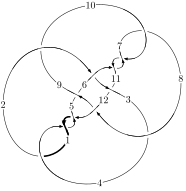
\includegraphics[width=112pt]{../../../GIT/diagram.site/Diagrams/png/1706_12a_0905.png}\\
\ \ \ A knot diagram\footnotemark}&
\allowdisplaybreaks
\textbf{Linearized knot diagam} \\
\cline{2-2}
 &
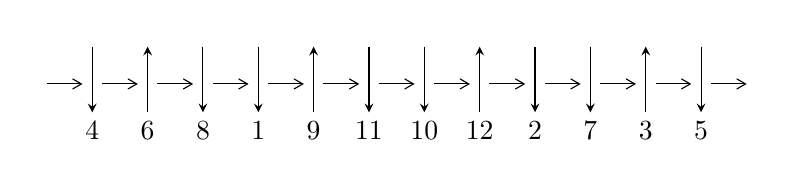
\begin{tikzpicture}[x=20pt, y=17pt]
	% nodes
	\node (C0) at (0, 0) {};
	\node (C1) at (1, 0) {};
	\node (C1U) at (1, +1) {};
	\node (C1D) at (1, -1) {4};

	\node (C2) at (2, 0) {};
	\node (C2U) at (2, +1) {};
	\node (C2D) at (2, -1) {6};

	\node (C3) at (3, 0) {};
	\node (C3U) at (3, +1) {};
	\node (C3D) at (3, -1) {8};

	\node (C4) at (4, 0) {};
	\node (C4U) at (4, +1) {};
	\node (C4D) at (4, -1) {1};

	\node (C5) at (5, 0) {};
	\node (C5U) at (5, +1) {};
	\node (C5D) at (5, -1) {9};

	\node (C6) at (6, 0) {};
	\node (C6U) at (6, +1) {};
	\node (C6D) at (6, -1) {11};

	\node (C7) at (7, 0) {};
	\node (C7U) at (7, +1) {};
	\node (C7D) at (7, -1) {10};

	\node (C8) at (8, 0) {};
	\node (C8U) at (8, +1) {};
	\node (C8D) at (8, -1) {12};

	\node (C9) at (9, 0) {};
	\node (C9U) at (9, +1) {};
	\node (C9D) at (9, -1) {2};

	\node (C10) at (10, 0) {};
	\node (C10U) at (10, +1) {};
	\node (C10D) at (10, -1) {7};

	\node (C11) at (11, 0) {};
	\node (C11U) at (11, +1) {};
	\node (C11D) at (11, -1) {3};

	\node (C12) at (12, 0) {};
	\node (C12U) at (12, +1) {};
	\node (C12D) at (12, -1) {5};
	\node (C13) at (13, 0) {};

	% arrows
	\draw[->,>={angle 60}]
	(C0) edge (C1) (C1) edge (C2) (C2) edge (C3) (C3) edge (C4) (C4) edge (C5) (C5) edge (C6) (C6) edge (C7) (C7) edge (C8) (C8) edge (C9) (C9) edge (C10) (C10) edge (C11) (C11) edge (C12) (C12) edge (C13) ;	\draw[->,>=stealth]
	(C1U) edge (C1D) (C2D) edge (C2U) (C3U) edge (C3D) (C4U) edge (C4D) (C5D) edge (C5U) (C6U) edge (C6D) (C7U) edge (C7D) (C8D) edge (C8U) (C9U) edge (C9D) (C10U) edge (C10D) (C11D) edge (C11U) (C12U) edge (C12D) ;
	\end{tikzpicture} \\
\hhline{~~} \\& 
\textbf{Solving Sequence} \\ \cline{2-2} 
 &
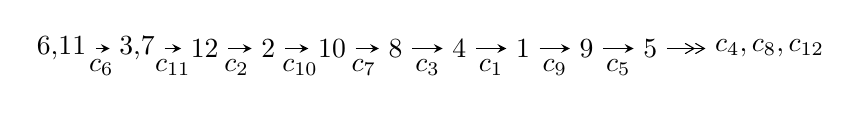
\begin{tikzpicture}[x=23pt, y=7pt]
	% node
	\node (A0) at (-1/8, 0) {6,11};
	\node (A1) at (17/16, 0) {3,7};
	\node (A2) at (17/8, 0) {12};
	\node (A3) at (25/8, 0) {2};
	\node (A4) at (33/8, 0) {10};
	\node (A5) at (41/8, 0) {8};
	\node (A6) at (49/8, 0) {4};
	\node (A7) at (57/8, 0) {1};
	\node (A8) at (65/8, 0) {9};
	\node (A9) at (73/8, 0) {5};
	\node (C1) at (1/2, -1) {$c_{6}$};
	\node (C2) at (13/8, -1) {$c_{11}$};
	\node (C3) at (21/8, -1) {$c_{2}$};
	\node (C4) at (29/8, -1) {$c_{10}$};
	\node (C5) at (37/8, -1) {$c_{7}$};
	\node (C6) at (45/8, -1) {$c_{3}$};
	\node (C7) at (53/8, -1) {$c_{1}$};
	\node (C8) at (61/8, -1) {$c_{9}$};
	\node (C9) at (69/8, -1) {$c_{5}$};
	\node (A10) at (11, 0) {$c_{4},c_{8},c_{12}$};

	% edge
	\draw[->,>=stealth]	
	(A0) edge (A1) (A1) edge (A2) (A2) edge (A3) (A3) edge (A4) (A4) edge (A5) (A5) edge (A6) (A6) edge (A7) (A7) edge (A8) (A8) edge (A9) ;
	\draw[->>,>={angle 60}]	
	(A9) edge (A10);
\end{tikzpicture} \\ 

\end{tabular} \\

\footnotetext{
The image of knot diagram is generated by the software ``\textbf{Draw programme}" developed by Andrew Bartholomew(\url{http://www.layer8.co.uk/maths/draw/index.htm\#Running-draw}), where we modified some parts for our purpose(\url{https://github.com/CATsTAILs/LinksPainter}).
}\phantom \\ \newline 
\centering \textbf{Ideals for irreducible components\footnotemark of $X_{\text{par}}$} 
 
\begin{align*}
I^u_{1}&=\langle 
- u^9- u^8-5 u^7-4 u^6-8 u^5-5 u^4-4 u^3- u^2+b- u+1,\;- u^{14}-3 u^{13}+\cdots+3 a+9,\\
\phantom{I^u_{1}}&\phantom{= \langle  }u^{15}+3 u^{14}+\cdots-6 u-3\rangle \\
I^u_{2}&=\langle 
-562052542293 u^{41}-4221685298499 u^{40}+\cdots+1614846925093 b+7465820808608,\\
\phantom{I^u_{2}}&\phantom{= \langle  }7465820808608 u^{41}+62536829180329 u^{40}+\cdots+8074234625465 a+154585802344000,\\
\phantom{I^u_{2}}&\phantom{= \langle  }u^{42}+8 u^{41}+\cdots+40 u+5\rangle \\
I^u_{3}&=\langle 
3 u^{23}-17 u^{22}+\cdots+b+4,\;4 u^{23} a-5 u^{23}+\cdots+9 a-20,\;u^{24}-5 u^{23}+\cdots+4 u+1\rangle \\
I^u_{4}&=\langle 
2 u^{21}-14 u^{20}+\cdots+b-3,\;3 u^{21}-19 u^{20}+\cdots+a-4,\;u^{22}-7 u^{21}+\cdots-8 u+1\rangle \\
I^u_{5}&=\langle 
- u^3- a u+u^2+b-2 u+1,\;u^3 a+u^3+a^2+2 a u+2 u+1,\;u^4- u^3+3 u^2-2 u+1\rangle \\
I^u_{6}&=\langle 
u^3- u^2+b+2 u-1,\;u^3+a+2 u,\;u^4- u^3+3 u^2-2 u+1\rangle \\
I^u_{7}&=\langle 
- a u- u^2+b+u-1,\;u^2 a+a^2- u^2+a-1,\;u^3- u^2+2 u-1\rangle \\
\\
I^v_{1}&=\langle 
a,\;b+1,\;v-1\rangle \\
\end{align*}
\raggedright * 8 irreducible components of $\dim_{\mathbb{C}}=0$, with total 146 representations.\\
\footnotetext{All coefficients of polynomials are rational numbers. But the coefficients are sometimes approximated in decimal forms when there is not enough margin.}
\newpage
\renewcommand{\arraystretch}{1}
\centering \section*{I. $I^u_{1}= \langle - u^9- u^8+\cdots+b+1,\;- u^{14}-3 u^{13}+\cdots+3 a+9,\;u^{15}+3 u^{14}+\cdots-6 u-3 \rangle$}
\flushleft \textbf{(i) Arc colorings}\\
\begin{tabular}{m{7pt} m{180pt} m{7pt} m{180pt} }
\flushright $a_{6}=$&$\begin{pmatrix}1\\0\end{pmatrix}$ \\
\flushright $a_{11}=$&$\begin{pmatrix}0\\u\end{pmatrix}$ \\
\flushright $a_{3}=$&$\begin{pmatrix}\frac{1}{3} u^{14}+u^{13}+\cdots-\frac{8}{3} u-3\\u^9+u^8+5 u^7+4 u^6+8 u^5+5 u^4+4 u^3+u^2+u-1\end{pmatrix}$ \\
\flushright $a_{7}=$&$\begin{pmatrix}1\\u^2\end{pmatrix}$ \\
\flushright $a_{12}=$&$\begin{pmatrix}\frac{1}{3} u^{14}+u^{13}+\cdots+\frac{1}{3} u-1\\u^{13}+2 u^{12}+\cdots-2 u^2-1\end{pmatrix}$ \\
\flushright $a_{2}=$&$\begin{pmatrix}\frac{1}{3} u^{14}+u^{13}+\cdots-\frac{11}{3} u-2\\u^9+u^8+5 u^7+4 u^6+8 u^5+5 u^4+4 u^3+u^2+u-1\end{pmatrix}$ \\
\flushright $a_{10}=$&$\begin{pmatrix}u\\u^3+u\end{pmatrix}$ \\
\flushright $a_{8}=$&$\begin{pmatrix}u^2+1\\u^4+2 u^2\end{pmatrix}$ \\
\flushright $a_{4}=$&$\begin{pmatrix}-\frac{2}{3} u^{14}- u^{13}+\cdots-\frac{5}{3} u-2\\- u^{13}-3 u^{12}+\cdots+4 u+2\end{pmatrix}$ \\
\flushright $a_{1}=$&$\begin{pmatrix}-\frac{2}{3} u^{14}-3 u^{13}+\cdots+\frac{13}{3} u^2+\frac{7}{3} u\\u^{14}+3 u^{13}+\cdots- u-1\end{pmatrix}$ \\
\flushright $a_{9}=$&$\begin{pmatrix}\frac{1}{3} u^{14}+u^{13}+\cdots-\frac{5}{3} u-1\\u^9+u^8+5 u^7+4 u^6+8 u^5+5 u^4+4 u^3+u^2+u-1\end{pmatrix}$ \\
\flushright $a_{5}=$&$\begin{pmatrix}-\frac{1}{3} u^{14}-\frac{1}{3} u^{12}+\cdots-\frac{1}{3} u^2-\frac{7}{3} u\\- u^{13}-2 u^{12}+\cdots+u+1\end{pmatrix}$\\&\end{tabular}
\flushleft \textbf{(ii) Obstruction class $= -1$}\\~\\
\flushleft \textbf{(iii) Cusp Shapes $= -2 u^{12}-6 u^{11}-22 u^{10}-44 u^9-84 u^8-120 u^7-142 u^6-144 u^5-102 u^4-64 u^3-20 u^2+6$}\\~\\
\newpage\renewcommand{\arraystretch}{1}
\flushleft \textbf{(iv) u-Polynomials at the component}\newline \\
\begin{tabular}{m{50pt}|m{274pt}}
Crossings & \hspace{64pt}u-Polynomials at each crossing \\
\hline $$\begin{aligned}c_{1},c_{4},c_{6}\\c_{7},c_{10},c_{12}\end{aligned}$$&$\begin{aligned}
&u^{15}-3 u^{14}+\cdots-6 u+3
\end{aligned}$\\
\hline $$\begin{aligned}c_{2},c_{5},c_{8}\\c_{11}\end{aligned}$$&$\begin{aligned}
&u^{15}+u^{14}+\cdots-7 u^2+1
\end{aligned}$\\
\hline $$\begin{aligned}c_{3},c_{9}\end{aligned}$$&$\begin{aligned}
&u^{15}-6 u^{14}+\cdots-24 u+8
\end{aligned}$\\
\hline
\end{tabular}\\~\\
\newpage\renewcommand{\arraystretch}{1}
\flushleft \textbf{(v) Riley Polynomials at the component}\newline \\
\begin{tabular}{m{50pt}|m{274pt}}
Crossings & \hspace{64pt}Riley Polynomials at each crossing \\
\hline $$\begin{aligned}c_{1},c_{4},c_{6}\\c_{7},c_{10},c_{12}\end{aligned}$$&$\begin{aligned}
&y^{15}+17 y^{14}+\cdots+6 y-9
\end{aligned}$\\
\hline $$\begin{aligned}c_{2},c_{5},c_{8}\\c_{11}\end{aligned}$$&$\begin{aligned}
&y^{15}-11 y^{14}+\cdots+14 y-1
\end{aligned}$\\
\hline $$\begin{aligned}c_{3},c_{9}\end{aligned}$$&$\begin{aligned}
&y^{15}-6 y^{14}+\cdots+224 y-64
\end{aligned}$\\
\hline
\end{tabular}\\~\\
\newpage\flushleft \textbf{(vi) Complex Volumes and Cusp Shapes}
$$\begin{array}{c|c|c}  
\text{Solutions to }I^u_{1}& \I (\text{vol} + \sqrt{-1}CS) & \text{Cusp shape}\\
 \hline 
\begin{aligned}
u &= -0.795561 + 0.469588 I \\
a &= \phantom{-}0.66756 + 1.38872 I \\
b &= \phantom{-}1.18321 + 0.79133 I\end{aligned}
 & \phantom{-}1.22894 + 9.98581 I & -2.50504 - 9.39516 I \\ \hline\begin{aligned}
u &= -0.795561 - 0.469588 I \\
a &= \phantom{-}0.66756 - 1.38872 I \\
b &= \phantom{-}1.18321 - 0.79133 I\end{aligned}
 & \phantom{-}1.22894 - 9.98581 I & -2.50504 + 9.39516 I \\ \hline\begin{aligned}
u &= \phantom{-}0.025319 + 0.816586 I \\
a &= -0.509860 - 0.477335 I \\
b &= -0.376877 + 0.428430 I\end{aligned}
 & \phantom{-}1.65484 - 1.30957 I & \phantom{-}1.85503 + 5.43942 I \\ \hline\begin{aligned}
u &= \phantom{-}0.025319 - 0.816586 I \\
a &= -0.509860 + 0.477335 I \\
b &= -0.376877 - 0.428430 I\end{aligned}
 & \phantom{-}1.65484 + 1.30957 I & \phantom{-}1.85503 - 5.43942 I \\ \hline\begin{aligned}
u &= -0.538585 + 0.452447 I \\
a &= -1.298690 - 0.499892 I \\
b &= -0.925630 + 0.318355 I\end{aligned}
 & \phantom{-}2.11810 - 0.75734 I & \phantom{-}1.216337 - 0.256399 I \\ \hline\begin{aligned}
u &= -0.538585 - 0.452447 I \\
a &= -1.298690 + 0.499892 I \\
b &= -0.925630 - 0.318355 I\end{aligned}
 & \phantom{-}2.11810 + 0.75734 I & \phantom{-}1.216337 + 0.256399 I \\ \hline\begin{aligned}
u &= \phantom{-}0.05955 + 1.44554 I \\
a &= -0.511356 + 0.845268 I \\
b &= \phantom{-}1.25232 + 0.68885 I\end{aligned}
 & \phantom{-}12.18430 - 0.89198 I & \phantom{-}5.76532 - 1.13067 I \\ \hline\begin{aligned}
u &= \phantom{-}0.05955 - 1.44554 I \\
a &= -0.511356 - 0.845268 I \\
b &= \phantom{-}1.25232 - 0.68885 I\end{aligned}
 & \phantom{-}12.18430 + 0.89198 I & \phantom{-}5.76532 + 1.13067 I \\ \hline\begin{aligned}
u &= \phantom{-}0.17394 + 1.44037 I \\
a &= \phantom{-}0.383006 - 0.328634 I \\
b &= -0.539974 - 0.494505 I\end{aligned}
 & \phantom{-}8.82530 - 4.42382 I & \phantom{-}1.11143 + 2.80902 I \\ \hline\begin{aligned}
u &= \phantom{-}0.17394 - 1.44037 I \\
a &= \phantom{-}0.383006 + 0.328634 I \\
b &= -0.539974 + 0.494505 I\end{aligned}
 & \phantom{-}8.82530 + 4.42382 I & \phantom{-}1.11143 - 2.80902 I\\
 \hline 
 \end{array}$$\newpage$$\begin{array}{c|c|c}  
\text{Solutions to }I^u_{1}& \I (\text{vol} + \sqrt{-1}CS) & \text{Cusp shape}\\
 \hline 
\begin{aligned}
u &= -0.34009 + 1.46037 I \\
a &= \phantom{-}0.223627 + 0.790180 I \\
b &= \phantom{-}1.230010 - 0.057843 I\end{aligned}
 & \phantom{-}13.5931 + 6.4489 I & \phantom{-}7.27407 - 4.21866 I \\ \hline\begin{aligned}
u &= -0.34009 - 1.46037 I \\
a &= \phantom{-}0.223627 - 0.790180 I \\
b &= \phantom{-}1.230010 + 0.057843 I\end{aligned}
 & \phantom{-}13.5931 - 6.4489 I & \phantom{-}7.27407 + 4.21866 I \\ \hline\begin{aligned}
u &= \phantom{-}0.436338\phantom{ +0.000000I} \\
a &= -0.713570\phantom{ +0.000000I} \\
b &= \phantom{-}0.311358\phantom{ +0.000000I}\end{aligned}
 & -0.991071\phantom{ +0.000000I} & -10.5830\phantom{ +0.000000I} \\ \hline\begin{aligned}
u &= -0.30274 + 1.53981 I \\
a &= \phantom{-}0.402502 - 1.039480 I \\
b &= -1.47873 - 0.93447 I\end{aligned}
 & \phantom{-}14.3514 + 18.1469 I & \phantom{-}3.57429 - 8.51279 I \\ \hline\begin{aligned}
u &= -0.30274 - 1.53981 I \\
a &= \phantom{-}0.402502 + 1.039480 I \\
b &= -1.47873 + 0.93447 I\end{aligned}
 & \phantom{-}14.3514 - 18.1469 I & \phantom{-}3.57429 + 8.51279 I\\
 \hline 
 \end{array}$$\newpage\newpage\renewcommand{\arraystretch}{1}
\centering \section*{II. $I^u_{2}= \langle -5.62\times10^{11} u^{41}-4.22\times10^{12} u^{40}+\cdots+1.61\times10^{12} b+7.47\times10^{12},\;7.47\times10^{12} u^{41}+6.25\times10^{13} u^{40}+\cdots+8.07\times10^{12} a+1.55\times10^{14},\;u^{42}+8 u^{41}+\cdots+40 u+5 \rangle$}
\flushleft \textbf{(i) Arc colorings}\\
\begin{tabular}{m{7pt} m{180pt} m{7pt} m{180pt} }
\flushright $a_{6}=$&$\begin{pmatrix}1\\0\end{pmatrix}$ \\
\flushright $a_{11}=$&$\begin{pmatrix}0\\u\end{pmatrix}$ \\
\flushright $a_{3}=$&$\begin{pmatrix}-0.924647 u^{41}-7.74523 u^{40}+\cdots-92.0620 u-19.1456\\0.348053 u^{41}+2.61429 u^{40}+\cdots-17.8403 u-4.62324\end{pmatrix}$ \\
\flushright $a_{7}=$&$\begin{pmatrix}1\\u^2\end{pmatrix}$ \\
\flushright $a_{12}=$&$\begin{pmatrix}0.0122164 u^{41}-0.389943 u^{40}+\cdots-63.7656 u-7.49795\\0.487674 u^{41}+5.20588 u^{40}+\cdots+8.98661 u+0.0610821\end{pmatrix}$ \\
\flushright $a_{2}=$&$\begin{pmatrix}-1.27270 u^{41}-10.3595 u^{40}+\cdots-74.2216 u-14.5223\\0.348053 u^{41}+2.61429 u^{40}+\cdots-17.8403 u-4.62324\end{pmatrix}$ \\
\flushright $a_{10}=$&$\begin{pmatrix}u\\u^3+u\end{pmatrix}$ \\
\flushright $a_{8}=$&$\begin{pmatrix}u^2+1\\u^4+2 u^2\end{pmatrix}$ \\
\flushright $a_{4}=$&$\begin{pmatrix}-0.836271 u^{41}-5.05200 u^{40}+\cdots-65.6783 u-14.8968\\-1.14490 u^{41}-9.64683 u^{40}+\cdots-56.7466 u-9.60670\end{pmatrix}$ \\
\flushright $a_{1}=$&$\begin{pmatrix}0.528605 u^{41}+3.36723 u^{40}+\cdots-8.24064 u-1.10136\\-0.314496 u^{41}-1.57614 u^{40}+\cdots-7.98768 u-1.64323\end{pmatrix}$ \\
\flushright $a_{9}=$&$\begin{pmatrix}0.261345 u^{41}+2.30222 u^{40}+\cdots+0.106070 u+1.77076\\-0.347361 u^{41}-2.64299 u^{40}+\cdots-3.78133 u-0.430082\end{pmatrix}$ \\
\flushright $a_{5}=$&$\begin{pmatrix}0.00701951 u^{41}+0.906686 u^{40}+\cdots+16.1301 u+2.32016\\-0.615275 u^{41}-4.95154 u^{40}+\cdots-14.9001 u-1.83426\end{pmatrix}$\\&\end{tabular}
\flushleft \textbf{(ii) Obstruction class $= -1$}\\~\\
\flushleft \textbf{(iii) Cusp Shapes $= \frac{11300023370492}{1614846925093} u^{41}+\frac{83794710538956}{1614846925093} u^{40}+\cdots+\frac{592947538978880}{1614846925093} u+\frac{103946797867048}{1614846925093}$}\\~\\
\newpage\renewcommand{\arraystretch}{1}
\flushleft \textbf{(iv) u-Polynomials at the component}\newline \\
\begin{tabular}{m{50pt}|m{274pt}}
Crossings & \hspace{64pt}u-Polynomials at each crossing \\
\hline $$\begin{aligned}c_{1},c_{4},c_{6}\\c_{7},c_{10},c_{12}\end{aligned}$$&$\begin{aligned}
&u^{42}-8 u^{41}+\cdots-40 u+5
\end{aligned}$\\
\hline $$\begin{aligned}c_{2},c_{5},c_{8}\\c_{11}\end{aligned}$$&$\begin{aligned}
&u^{42}-13 u^{40}+\cdots- u+1
\end{aligned}$\\
\hline $$\begin{aligned}c_{3},c_{9}\end{aligned}$$&$\begin{aligned}
&(u^{21}+3 u^{20}+\cdots- u-5)^{2}
\end{aligned}$\\
\hline
\end{tabular}\\~\\
\newpage\renewcommand{\arraystretch}{1}
\flushleft \textbf{(v) Riley Polynomials at the component}\newline \\
\begin{tabular}{m{50pt}|m{274pt}}
Crossings & \hspace{64pt}Riley Polynomials at each crossing \\
\hline $$\begin{aligned}c_{1},c_{4},c_{6}\\c_{7},c_{10},c_{12}\end{aligned}$$&$\begin{aligned}
&y^{42}+40 y^{41}+\cdots+100 y+25
\end{aligned}$\\
\hline $$\begin{aligned}c_{2},c_{5},c_{8}\\c_{11}\end{aligned}$$&$\begin{aligned}
&y^{42}-26 y^{41}+\cdots-127 y+1
\end{aligned}$\\
\hline $$\begin{aligned}c_{3},c_{9}\end{aligned}$$&$\begin{aligned}
&(y^{21}+9 y^{20}+\cdots-319 y-25)^{2}
\end{aligned}$\\
\hline
\end{tabular}\\~\\
\newpage\flushleft \textbf{(vi) Complex Volumes and Cusp Shapes}
$$\begin{array}{c|c|c}  
\text{Solutions to }I^u_{2}& \I (\text{vol} + \sqrt{-1}CS) & \text{Cusp shape}\\
 \hline 
\begin{aligned}
u &= -0.853330 + 0.522684 I \\
a &= -0.59606 - 1.28608 I \\
b &= -1.18084 - 0.78590 I\end{aligned}
 & \phantom{-}7.6520 + 13.9242 I & \phantom{-0.000000 } 0. - 8.90479 I \\ \hline\begin{aligned}
u &= -0.853330 - 0.522684 I \\
a &= -0.59606 + 1.28608 I \\
b &= -1.18084 + 0.78590 I\end{aligned}
 & \phantom{-}7.6520 - 13.9242 I & \phantom{-0.000000 -}0. + 8.90479 I \\ \hline\begin{aligned}
u &= -0.712897 + 0.659919 I \\
a &= \phantom{-}1.002160 + 0.322440 I \\
b &= \phantom{-}0.927217 - 0.431475 I\end{aligned}
 & \phantom{-}1.79638 - 4.88565 I & \phantom{-0.000000 -}0. + 5.93325 I \\ \hline\begin{aligned}
u &= -0.712897 - 0.659919 I \\
a &= \phantom{-}1.002160 - 0.322440 I \\
b &= \phantom{-}0.927217 + 0.431475 I\end{aligned}
 & \phantom{-}1.79638 + 4.88565 I & \phantom{-0.000000 } 0. - 5.93325 I \\ \hline\begin{aligned}
u &= \phantom{-}0.593838 + 0.841447 I \\
a &= -0.112224 + 0.107302 I \\
b &= \phantom{-}0.156931 + 0.030710 I\end{aligned}
 & -0.50781 - 2.31740 I & \phantom{-0.000000 } 0 \\ \hline\begin{aligned}
u &= \phantom{-}0.593838 - 0.841447 I \\
a &= -0.112224 - 0.107302 I \\
b &= \phantom{-}0.156931 - 0.030710 I\end{aligned}
 & -0.50781 + 2.31740 I & \phantom{-0.000000 } 0 \\ \hline\begin{aligned}
u &= -0.839691 + 0.678343 I \\
a &= -0.943185 - 0.221439 I \\
b &= -0.942195 + 0.453863 I\end{aligned}
 & \phantom{-}8.04725 - 8.28146 I & \phantom{-0.000000 } 0 \\ \hline\begin{aligned}
u &= -0.839691 - 0.678343 I \\
a &= -0.943185 + 0.221439 I \\
b &= -0.942195 - 0.453863 I\end{aligned}
 & \phantom{-}8.04725 + 8.28146 I & \phantom{-0.000000 } 0 \\ \hline\begin{aligned}
u &= \phantom{-}0.731574 + 0.444637 I \\
a &= \phantom{-}0.267734 - 0.175635 I \\
b &= -0.273961 + 0.009446 I\end{aligned}
 & \phantom{-}2.78697 - 1.47830 I & -3.32231 + 0.64878 I \\ \hline\begin{aligned}
u &= \phantom{-}0.731574 - 0.444637 I \\
a &= \phantom{-}0.267734 + 0.175635 I \\
b &= -0.273961 - 0.009446 I\end{aligned}
 & \phantom{-}2.78697 + 1.47830 I & -3.32231 - 0.64878 I\\
 \hline 
 \end{array}$$\newpage$$\begin{array}{c|c|c}  
\text{Solutions to }I^u_{2}& \I (\text{vol} + \sqrt{-1}CS) & \text{Cusp shape}\\
 \hline 
\begin{aligned}
u &= -0.775939 + 0.274659 I \\
a &= \phantom{-}1.401210 - 0.008524 I \\
b &= \phantom{-}1.084910 - 0.391468 I\end{aligned}
 & \phantom{-}8.03896 + 2.27731 I & \phantom{-}3.60405 - 1.97458 I \\ \hline\begin{aligned}
u &= -0.775939 - 0.274659 I \\
a &= \phantom{-}1.401210 + 0.008524 I \\
b &= \phantom{-}1.084910 + 0.391468 I\end{aligned}
 & \phantom{-}8.03896 - 2.27731 I & \phantom{-}3.60405 + 1.97458 I \\ \hline\begin{aligned}
u &= -0.682700 + 0.436541 I \\
a &= -0.67403 - 1.62063 I \\
b &= -1.16763 - 0.81216 I\end{aligned}
 & \phantom{-}1.79638 + 4.88565 I & -0.60467 - 5.93325 I \\ \hline\begin{aligned}
u &= -0.682700 - 0.436541 I \\
a &= -0.67403 + 1.62063 I \\
b &= -1.16763 + 0.81216 I\end{aligned}
 & \phantom{-}1.79638 - 4.88565 I & -0.60467 + 5.93325 I \\ \hline\begin{aligned}
u &= -0.518391 + 0.574589 I \\
a &= \phantom{-}0.25967 + 1.72822 I \\
b &= \phantom{-}1.127630 + 0.746695 I\end{aligned}
 & \phantom{-}9.22998 + 1.82910 I & \phantom{-}4.46798 - 3.91898 I \\ \hline\begin{aligned}
u &= -0.518391 - 0.574589 I \\
a &= \phantom{-}0.25967 - 1.72822 I \\
b &= \phantom{-}1.127630 - 0.746695 I\end{aligned}
 & \phantom{-}9.22998 - 1.82910 I & \phantom{-}4.46798 + 3.91898 I \\ \hline\begin{aligned}
u &= \phantom{-}0.682538 + 1.019720 I \\
a &= \phantom{-}0.179954 - 0.091678 I \\
b &= -0.216311 - 0.120929 I\end{aligned}
 & \phantom{-}4.29895 - 3.75943 I & \phantom{-0.000000 } 0 \\ \hline\begin{aligned}
u &= \phantom{-}0.682538 - 1.019720 I \\
a &= \phantom{-}0.179954 + 0.091678 I \\
b &= -0.216311 + 0.120929 I\end{aligned}
 & \phantom{-}4.29895 + 3.75943 I & \phantom{-0.000000 } 0 \\ \hline\begin{aligned}
u &= -0.052768 + 1.314890 I \\
a &= -0.355444 + 0.977726 I \\
b &= \phantom{-}1.266840 + 0.518962 I\end{aligned}
 & \phantom{-}10.2049\phantom{ +0.000000I} & \phantom{-0.000000 } 0 \\ \hline\begin{aligned}
u &= -0.052768 - 1.314890 I \\
a &= -0.355444 - 0.977726 I \\
b &= \phantom{-}1.266840 - 0.518962 I\end{aligned}
 & \phantom{-}10.2049\phantom{ +0.000000I} & \phantom{-0.000000 } 0\\
 \hline 
 \end{array}$$\newpage$$\begin{array}{c|c|c}  
\text{Solutions to }I^u_{2}& \I (\text{vol} + \sqrt{-1}CS) & \text{Cusp shape}\\
 \hline 
\begin{aligned}
u &= \phantom{-}0.027560 + 1.319270 I \\
a &= -0.706441 + 0.342428 I \\
b &= \phantom{-}0.471226 + 0.922552 I\end{aligned}
 & \phantom{-}2.78697 - 1.47830 I & \phantom{-0.000000 } 0 \\ \hline\begin{aligned}
u &= \phantom{-}0.027560 - 1.319270 I \\
a &= -0.706441 - 0.342428 I \\
b &= \phantom{-}0.471226 - 0.922552 I\end{aligned}
 & \phantom{-}2.78697 + 1.47830 I & \phantom{-0.000000 } 0 \\ \hline\begin{aligned}
u &= -0.082150 + 1.381150 I \\
a &= \phantom{-}0.871679 - 0.724775 I \\
b &= -0.92941 - 1.26346 I\end{aligned}
 & \phantom{-}4.29895 + 3.75943 I & \phantom{-0.000000 } 0 \\ \hline\begin{aligned}
u &= -0.082150 - 1.381150 I \\
a &= \phantom{-}0.871679 + 0.724775 I \\
b &= -0.92941 + 1.26346 I\end{aligned}
 & \phantom{-}4.29895 - 3.75943 I & \phantom{-0.000000 } 0 \\ \hline\begin{aligned}
u &= \phantom{-}0.014975 + 1.414050 I \\
a &= \phantom{-}0.451593 - 0.837497 I \\
b &= -1.191030 - 0.626035 I\end{aligned}
 & \phantom{-}6.62865 - 0.11622 I & \phantom{-0.000000 } 0 \\ \hline\begin{aligned}
u &= \phantom{-}0.014975 - 1.414050 I \\
a &= \phantom{-}0.451593 + 0.837497 I \\
b &= -1.191030 + 0.626035 I\end{aligned}
 & \phantom{-}6.62865 + 0.11622 I & \phantom{-0.000000 } 0 \\ \hline\begin{aligned}
u &= -0.25079 + 1.45386 I \\
a &= -0.056197 - 0.851127 I \\
b &= -1.251510 - 0.131755 I\end{aligned}
 & \phantom{-}8.03896 + 2.27731 I & \phantom{-0.000000 } 0 \\ \hline\begin{aligned}
u &= -0.25079 - 1.45386 I \\
a &= -0.056197 + 0.851127 I \\
b &= -1.251510 + 0.131755 I\end{aligned}
 & \phantom{-}8.03896 - 2.27731 I & \phantom{-0.000000 } 0 \\ \hline\begin{aligned}
u &= -0.24529 + 1.48742 I \\
a &= \phantom{-}0.492155 - 1.095830 I \\
b &= -1.50924 - 1.00084 I\end{aligned}
 & \phantom{-}8.04725 + 8.28146 I & \phantom{-0.000000 } 0 \\ \hline\begin{aligned}
u &= -0.24529 - 1.48742 I \\
a &= \phantom{-}0.492155 + 1.095830 I \\
b &= -1.50924 + 1.00084 I\end{aligned}
 & \phantom{-}8.04725 - 8.28146 I & \phantom{-0.000000 } 0\\
 \hline 
 \end{array}$$\newpage$$\begin{array}{c|c|c}  
\text{Solutions to }I^u_{2}& \I (\text{vol} + \sqrt{-1}CS) & \text{Cusp shape}\\
 \hline 
\begin{aligned}
u &= -0.17608 + 1.50947 I \\
a &= -0.565601 + 0.999475 I \\
b &= \phantom{-}1.40909 + 1.02974 I\end{aligned}
 & \phantom{-}16.0135 + 4.3954 I & \phantom{-0.000000 } 0 \\ \hline\begin{aligned}
u &= -0.17608 - 1.50947 I \\
a &= -0.565601 - 0.999475 I \\
b &= \phantom{-}1.40909 - 1.02974 I\end{aligned}
 & \phantom{-}16.0135 - 4.3954 I & \phantom{-0.000000 } 0 \\ \hline\begin{aligned}
u &= -0.28548 + 1.51045 I \\
a &= -0.425571 + 1.072440 I \\
b &= \phantom{-}1.49838 + 0.94896 I\end{aligned}
 & \phantom{-}7.6520 + 13.9242 I & \phantom{-0.000000 } 0 \\ \hline\begin{aligned}
u &= -0.28548 - 1.51045 I \\
a &= -0.425571 - 1.072440 I \\
b &= \phantom{-}1.49838 - 0.94896 I\end{aligned}
 & \phantom{-}7.6520 - 13.9242 I & \phantom{-0.000000 } 0 \\ \hline\begin{aligned}
u &= -0.16988 + 1.54466 I \\
a &= -0.058448 + 0.687065 I \\
b &= \phantom{-}1.051350 + 0.207003 I\end{aligned}
 & \phantom{-}9.22998 - 1.82910 I & \phantom{-0.000000 } 0 \\ \hline\begin{aligned}
u &= -0.16988 - 1.54466 I \\
a &= -0.058448 - 0.687065 I \\
b &= \phantom{-}1.051350 - 0.207003 I\end{aligned}
 & \phantom{-}9.22998 + 1.82910 I & \phantom{-0.000000 } 0 \\ \hline\begin{aligned}
u &= -0.348258 + 0.115828 I \\
a &= -0.24840 - 3.12015 I \\
b &= -0.447909 - 1.057840 I\end{aligned}
 & -0.50781 + 2.31740 I & -1.63390 + 8.03476 I \\ \hline\begin{aligned}
u &= -0.348258 - 0.115828 I \\
a &= -0.24840 + 3.12015 I \\
b &= -0.447909 + 1.057840 I\end{aligned}
 & -0.50781 - 2.31740 I & -1.63390 - 8.03476 I \\ \hline\begin{aligned}
u &= -0.19258 + 1.63607 I \\
a &= \phantom{-}0.008104 - 0.588711 I \\
b &= -0.961610 - 0.126633 I\end{aligned}
 & \phantom{-}16.0135 - 4.3954 I & \phantom{-0.000000 } 0 \\ \hline\begin{aligned}
u &= -0.19258 - 1.63607 I \\
a &= \phantom{-}0.008104 + 0.588711 I \\
b &= -0.961610 + 0.126633 I\end{aligned}
 & \phantom{-}16.0135 + 4.3954 I & \phantom{-0.000000 } 0\\
 \hline 
 \end{array}$$\newpage$$\begin{array}{c|c|c}  
\text{Solutions to }I^u_{2}& \I (\text{vol} + \sqrt{-1}CS) & \text{Cusp shape}\\
 \hline 
\begin{aligned}
u &= \phantom{-}0.135742 + 0.185761 I \\
a &= -3.19264 + 3.47066 I \\
b &= \phantom{-}1.078090 + 0.121956 I\end{aligned}
 & \phantom{-}6.62865 - 0.11622 I & \phantom{-}5.95241 - 0.33252 I \\ \hline\begin{aligned}
u &= \phantom{-}0.135742 - 0.185761 I \\
a &= -3.19264 - 3.47066 I \\
b &= \phantom{-}1.078090 - 0.121956 I\end{aligned}
 & \phantom{-}6.62865 + 0.11622 I & \phantom{-}5.95241 + 0.33252 I\\
 \hline 
 \end{array}$$\newpage\newpage\renewcommand{\arraystretch}{1}
\centering \section*{III. $I^u_{3}= \langle 3 u^{23}-17 u^{22}+\cdots+b+4,\;4 u^{23} a-5 u^{23}+\cdots+9 a-20,\;u^{24}-5 u^{23}+\cdots+4 u+1 \rangle$}
\flushleft \textbf{(i) Arc colorings}\\
\begin{tabular}{m{7pt} m{180pt} m{7pt} m{180pt} }
\flushright $a_{6}=$&$\begin{pmatrix}1\\0\end{pmatrix}$ \\
\flushright $a_{11}=$&$\begin{pmatrix}0\\u\end{pmatrix}$ \\
\flushright $a_{3}=$&$\begin{pmatrix}a\\-3 u^{23}+17 u^{22}+\cdots-7 u-4\end{pmatrix}$ \\
\flushright $a_{7}=$&$\begin{pmatrix}1\\u^2\end{pmatrix}$ \\
\flushright $a_{12}=$&$\begin{pmatrix}3 u^{23} a- u^{23}+\cdots+4 a-5\\1\end{pmatrix}$ \\
\flushright $a_{2}=$&$\begin{pmatrix}3 u^{23}-17 u^{22}+\cdots+a+4\\-3 u^{23}+17 u^{22}+\cdots-7 u-4\end{pmatrix}$ \\
\flushright $a_{10}=$&$\begin{pmatrix}u\\u^3+u\end{pmatrix}$ \\
\flushright $a_{8}=$&$\begin{pmatrix}u^2+1\\u^4+2 u^2\end{pmatrix}$ \\
\flushright $a_{4}=$&$\begin{pmatrix}3 u^{23}-17 u^{22}+\cdots+a+6\\-2 u^{23}+11 u^{22}+\cdots-4 u-2\end{pmatrix}$ \\
\flushright $a_{1}=$&$\begin{pmatrix}- u^{23}+5 u^{22}+\cdots+a-5\\- u^{16} a+u^{16}+\cdots+a u+1\end{pmatrix}$ \\
\flushright $a_{9}=$&$\begin{pmatrix}2 u^{23} a- u^{23}+\cdots+4 a-6\\u^{21} a-6 u^{20} a+\cdots+2 a-1\end{pmatrix}$ \\
\flushright $a_{5}=$&$\begin{pmatrix}- u^{22} a- u^{23}+\cdots- a-5\\u^{17} a-3 u^{16} a+\cdots+a+1\end{pmatrix}$\\&\end{tabular}
\flushleft \textbf{(ii) Obstruction class $= -1$}\\~\\
\flushleft \textbf{(iii) Cusp Shapes $= -8 u^{23}+48 u^{22}-232 u^{21}+784 u^{20}-2224 u^{19}+5216 u^{18}-10568 u^{17}+18508 u^{16}-28364 u^{15}+37944 u^{14}-44324 u^{13}+44672 u^{12}-38328 u^{11}+27016 u^{10}-14640 u^9+4908 u^8+232 u^7-1516 u^6+800 u^5-8 u^4-232 u^3+120 u^2-16 u-38$}\\~\\
\newpage\renewcommand{\arraystretch}{1}
\flushleft \textbf{(iv) u-Polynomials at the component}\newline \\
\begin{tabular}{m{50pt}|m{274pt}}
Crossings & \hspace{64pt}u-Polynomials at each crossing \\
\hline $$\begin{aligned}c_{1},c_{4},c_{6}\\c_{7},c_{10},c_{12}\end{aligned}$$&$\begin{aligned}
&(u^{24}+5 u^{23}+\cdots-4 u+1)^{2}
\end{aligned}$\\
\hline $$\begin{aligned}c_{2},c_{5},c_{8}\\c_{11}\end{aligned}$$&$\begin{aligned}
&u^{48}- u^{47}+\cdots+36 u+61
\end{aligned}$\\
\hline $$\begin{aligned}c_{3},c_{9}\end{aligned}$$&$\begin{aligned}
&(u^{24}+u^{23}+\cdots-44 u+8)^{2}
\end{aligned}$\\
\hline
\end{tabular}\\~\\
\newpage\renewcommand{\arraystretch}{1}
\flushleft \textbf{(v) Riley Polynomials at the component}\newline \\
\begin{tabular}{m{50pt}|m{274pt}}
Crossings & \hspace{64pt}Riley Polynomials at each crossing \\
\hline $$\begin{aligned}c_{1},c_{4},c_{6}\\c_{7},c_{10},c_{12}\end{aligned}$$&$\begin{aligned}
&(y^{24}+23 y^{23}+\cdots-16 y+1)^{2}
\end{aligned}$\\
\hline $$\begin{aligned}c_{2},c_{5},c_{8}\\c_{11}\end{aligned}$$&$\begin{aligned}
&y^{48}+17 y^{47}+\cdots-19840 y+3721
\end{aligned}$\\
\hline $$\begin{aligned}c_{3},c_{9}\end{aligned}$$&$\begin{aligned}
&(y^{24}+9 y^{23}+\cdots-1040 y+64)^{2}
\end{aligned}$\\
\hline
\end{tabular}\\~\\
\newpage\flushleft \textbf{(vi) Complex Volumes and Cusp Shapes}
$$\begin{array}{c|c|c}  
\text{Solutions to }I^u_{3}& \I (\text{vol} + \sqrt{-1}CS) & \text{Cusp shape}\\
 \hline 
\begin{aligned}
u &= \phantom{-}0.800271 + 0.533236 I \\
a &= -0.422845 + 0.739232 I \\
b &= -0.509225 + 0.473403 I\end{aligned}
 & -0.96728 - 2.64620 I & -16.0316 + 9.3014 I \\ \hline\begin{aligned}
u &= \phantom{-}0.800271 + 0.533236 I \\
a &= \phantom{-}0.167698 - 0.703293 I \\
b &= \phantom{-}0.732576 - 0.366110 I\end{aligned}
 & -0.96728 - 2.64620 I & -16.0316 + 9.3014 I \\ \hline\begin{aligned}
u &= \phantom{-}0.800271 - 0.533236 I \\
a &= -0.422845 - 0.739232 I \\
b &= -0.509225 - 0.473403 I\end{aligned}
 & -0.96728 + 2.64620 I & -16.0316 - 9.3014 I \\ \hline\begin{aligned}
u &= \phantom{-}0.800271 - 0.533236 I \\
a &= \phantom{-}0.167698 + 0.703293 I \\
b &= \phantom{-}0.732576 + 0.366110 I\end{aligned}
 & -0.96728 + 2.64620 I & -16.0316 - 9.3014 I \\ \hline\begin{aligned}
u &= \phantom{-}0.878799 + 0.336754 I \\
a &= \phantom{-}0.630433 - 0.599955 I \\
b &= \phantom{-}0.294705 - 0.322645 I\end{aligned}
 & \phantom{-}2.66736 - 1.66203 I & -6.75738 + 1.82032 I \\ \hline\begin{aligned}
u &= \phantom{-}0.878799 + 0.336754 I \\
a &= -0.169737 + 0.432187 I \\
b &= -0.756061 + 0.314940 I\end{aligned}
 & \phantom{-}2.66736 - 1.66203 I & -6.75738 + 1.82032 I \\ \hline\begin{aligned}
u &= \phantom{-}0.878799 - 0.336754 I \\
a &= \phantom{-}0.630433 + 0.599955 I \\
b &= \phantom{-}0.294705 + 0.322645 I\end{aligned}
 & \phantom{-}2.66736 + 1.66203 I & -6.75738 - 1.82032 I \\ \hline\begin{aligned}
u &= \phantom{-}0.878799 - 0.336754 I \\
a &= -0.169737 - 0.432187 I \\
b &= -0.756061 - 0.314940 I\end{aligned}
 & \phantom{-}2.66736 + 1.66203 I & -6.75738 - 1.82032 I \\ \hline\begin{aligned}
u &= \phantom{-}0.832655 + 0.672098 I \\
a &= \phantom{-}0.367542 - 0.698741 I \\
b &= \phantom{-}0.497125 - 0.651920 I\end{aligned}
 & \phantom{-}3.62403 - 3.95529 I & -3.21624 + 9.39142 I \\ \hline\begin{aligned}
u &= \phantom{-}0.832655 + 0.672098 I \\
a &= \phantom{-}0.021153 + 0.765867 I \\
b &= -0.775658 + 0.334786 I\end{aligned}
 & \phantom{-}3.62403 - 3.95529 I & -3.21624 + 9.39142 I\\
 \hline 
 \end{array}$$\newpage$$\begin{array}{c|c|c}  
\text{Solutions to }I^u_{3}& \I (\text{vol} + \sqrt{-1}CS) & \text{Cusp shape}\\
 \hline 
\begin{aligned}
u &= \phantom{-}0.832655 - 0.672098 I \\
a &= \phantom{-}0.367542 + 0.698741 I \\
b &= \phantom{-}0.497125 + 0.651920 I\end{aligned}
 & \phantom{-}3.62403 + 3.95529 I & -3.21624 - 9.39142 I \\ \hline\begin{aligned}
u &= \phantom{-}0.832655 - 0.672098 I \\
a &= \phantom{-}0.021153 - 0.765867 I \\
b &= -0.775658 - 0.334786 I\end{aligned}
 & \phantom{-}3.62403 + 3.95529 I & -3.21624 - 9.39142 I \\ \hline\begin{aligned}
u &= \phantom{-}0.086298 + 0.746831 I \\
a &= \phantom{-}0.376144 - 1.063920 I \\
b &= \phantom{-}0.853689 - 1.098230 I\end{aligned}
 & \phantom{-}7.62597 - 5.15237 I & \phantom{-}5.88005 + 4.48367 I \\ \hline\begin{aligned}
u &= \phantom{-}0.086298 + 0.746831 I \\
a &= \phantom{-}1.32079 + 1.29570 I \\
b &= -0.827028 - 0.189102 I\end{aligned}
 & \phantom{-}7.62597 - 5.15237 I & \phantom{-}5.88005 + 4.48367 I \\ \hline\begin{aligned}
u &= \phantom{-}0.086298 - 0.746831 I \\
a &= \phantom{-}0.376144 + 1.063920 I \\
b &= \phantom{-}0.853689 + 1.098230 I\end{aligned}
 & \phantom{-}7.62597 + 5.15237 I & \phantom{-}5.88005 - 4.48367 I \\ \hline\begin{aligned}
u &= \phantom{-}0.086298 - 0.746831 I \\
a &= \phantom{-}1.32079 - 1.29570 I \\
b &= -0.827028 + 0.189102 I\end{aligned}
 & \phantom{-}7.62597 + 5.15237 I & \phantom{-}5.88005 - 4.48367 I \\ \hline\begin{aligned}
u &= \phantom{-}0.001993 + 1.316790 I \\
a &= -0.714558 - 0.020052 I \\
b &= \phantom{-}1.42656 + 1.02275 I\end{aligned}
 & \phantom{-}2.66736 - 1.66203 I & -6.75738 + 1.82032 I \\ \hline\begin{aligned}
u &= \phantom{-}0.001993 + 1.316790 I \\
a &= -0.778333 + 1.082180 I \\
b &= -0.024981 + 0.940966 I\end{aligned}
 & \phantom{-}2.66736 - 1.66203 I & -6.75738 + 1.82032 I \\ \hline\begin{aligned}
u &= \phantom{-}0.001993 - 1.316790 I \\
a &= -0.714558 + 0.020052 I \\
b &= \phantom{-}1.42656 - 1.02275 I\end{aligned}
 & \phantom{-}2.66736 + 1.66203 I & -6.75738 - 1.82032 I \\ \hline\begin{aligned}
u &= \phantom{-}0.001993 - 1.316790 I \\
a &= -0.778333 - 1.082180 I \\
b &= -0.024981 - 0.940966 I\end{aligned}
 & \phantom{-}2.66736 + 1.66203 I & -6.75738 - 1.82032 I\\
 \hline 
 \end{array}$$\newpage$$\begin{array}{c|c|c}  
\text{Solutions to }I^u_{3}& \I (\text{vol} + \sqrt{-1}CS) & \text{Cusp shape}\\
 \hline 
\begin{aligned}
u &= -0.066677 + 1.368660 I \\
a &= \phantom{-}0.347208 - 0.433644 I \\
b &= -0.14080 - 2.27520 I\end{aligned}
 & \phantom{-}3.62403 + 3.95529 I & -3.21624 - 9.39142 I \\ \hline\begin{aligned}
u &= -0.066677 + 1.368660 I \\
a &= \phantom{-}1.65342 - 0.18342 I \\
b &= -0.570359 - 0.504124 I\end{aligned}
 & \phantom{-}3.62403 + 3.95529 I & -3.21624 - 9.39142 I \\ \hline\begin{aligned}
u &= -0.066677 - 1.368660 I \\
a &= \phantom{-}0.347208 + 0.433644 I \\
b &= -0.14080 + 2.27520 I\end{aligned}
 & \phantom{-}3.62403 - 3.95529 I & -3.21624 + 9.39142 I \\ \hline\begin{aligned}
u &= -0.066677 - 1.368660 I \\
a &= \phantom{-}1.65342 + 0.18342 I \\
b &= -0.570359 + 0.504124 I\end{aligned}
 & \phantom{-}3.62403 - 3.95529 I & -3.21624 + 9.39142 I \\ \hline\begin{aligned}
u &= -0.09853 + 1.41543 I \\
a &= -0.177972 + 0.481724 I \\
b &= -0.57639 + 2.39043 I\end{aligned}
 & \phantom{-}10.95020 + 8.21862 I & \phantom{-}4.30637 - 9.35603 I \\ \hline\begin{aligned}
u &= -0.09853 + 1.41543 I \\
a &= -1.70890 - 0.28826 I \\
b &= \phantom{-}0.664312 + 0.299373 I\end{aligned}
 & \phantom{-}10.95020 + 8.21862 I & \phantom{-}4.30637 - 9.35603 I \\ \hline\begin{aligned}
u &= -0.09853 - 1.41543 I \\
a &= -0.177972 - 0.481724 I \\
b &= -0.57639 - 2.39043 I\end{aligned}
 & \phantom{-}10.95020 - 8.21862 I & \phantom{-}4.30637 + 9.35603 I \\ \hline\begin{aligned}
u &= -0.09853 - 1.41543 I \\
a &= -1.70890 + 0.28826 I \\
b &= \phantom{-}0.664312 - 0.299373 I\end{aligned}
 & \phantom{-}10.95020 - 8.21862 I & \phantom{-}4.30637 + 9.35603 I \\ \hline\begin{aligned}
u &= \phantom{-}0.18804 + 1.48037 I \\
a &= -0.334661 - 1.114890 I \\
b &= \phantom{-}0.773120 - 0.589137 I\end{aligned}
 & \phantom{-}7.62597 - 5.15237 I & \phantom{-}5.88005 + 4.48367 I \\ \hline\begin{aligned}
u &= \phantom{-}0.18804 + 1.48037 I \\
a &= \phantom{-}0.326363 + 0.563705 I \\
b &= -1.58751 + 0.70507 I\end{aligned}
 & \phantom{-}7.62597 - 5.15237 I & \phantom{-}5.88005 + 4.48367 I\\
 \hline 
 \end{array}$$\newpage$$\begin{array}{c|c|c}  
\text{Solutions to }I^u_{3}& \I (\text{vol} + \sqrt{-1}CS) & \text{Cusp shape}\\
 \hline 
\begin{aligned}
u &= \phantom{-}0.18804 - 1.48037 I \\
a &= -0.334661 + 1.114890 I \\
b &= \phantom{-}0.773120 + 0.589137 I\end{aligned}
 & \phantom{-}7.62597 + 5.15237 I & \phantom{-}5.88005 - 4.48367 I \\ \hline\begin{aligned}
u &= \phantom{-}0.18804 - 1.48037 I \\
a &= \phantom{-}0.326363 - 0.563705 I \\
b &= -1.58751 - 0.70507 I\end{aligned}
 & \phantom{-}7.62597 + 5.15237 I & \phantom{-}5.88005 - 4.48367 I \\ \hline\begin{aligned}
u &= \phantom{-}0.28419 + 1.52691 I \\
a &= -0.420040 - 0.724771 I \\
b &= \phantom{-}1.181840 - 0.532265 I\end{aligned}
 & \phantom{-}5.70851 - 6.62112 I & -4.00000 + 11.74539 I \\ \hline\begin{aligned}
u &= \phantom{-}0.28419 + 1.52691 I \\
a &= \phantom{-}0.197684 + 0.810796 I \\
b &= -0.987293 + 0.847336 I\end{aligned}
 & \phantom{-}5.70851 - 6.62112 I & -4.00000 + 11.74539 I \\ \hline\begin{aligned}
u &= \phantom{-}0.28419 - 1.52691 I \\
a &= -0.420040 + 0.724771 I \\
b &= \phantom{-}1.181840 + 0.532265 I\end{aligned}
 & \phantom{-}5.70851 + 6.62112 I & -4.00000 - 11.74539 I \\ \hline\begin{aligned}
u &= \phantom{-}0.28419 - 1.52691 I \\
a &= \phantom{-}0.197684 - 0.810796 I \\
b &= -0.987293 - 0.847336 I\end{aligned}
 & \phantom{-}5.70851 + 6.62112 I & -4.00000 - 11.74539 I \\ \hline\begin{aligned}
u &= -0.372821 + 0.191675 I \\
a &= \phantom{-}0.20434 + 2.08277 I \\
b &= -0.66433 + 1.43354 I\end{aligned}
 & \phantom{-}5.70851 + 6.62112 I & -4.18117 - 11.74539 I \\ \hline\begin{aligned}
u &= -0.372821 + 0.191675 I \\
a &= -2.97294 + 2.31667 I \\
b &= \phantom{-}0.475400 + 0.737334 I\end{aligned}
 & \phantom{-}5.70851 + 6.62112 I & -4.18117 - 11.74539 I \\ \hline\begin{aligned}
u &= -0.372821 - 0.191675 I \\
a &= \phantom{-}0.20434 - 2.08277 I \\
b &= -0.66433 - 1.43354 I\end{aligned}
 & \phantom{-}5.70851 - 6.62112 I & -4.18117 + 11.74539 I \\ \hline\begin{aligned}
u &= -0.372821 - 0.191675 I \\
a &= -2.97294 - 2.31667 I \\
b &= \phantom{-}0.475400 - 0.737334 I\end{aligned}
 & \phantom{-}5.70851 - 6.62112 I & -4.18117 + 11.74539 I\\
 \hline 
 \end{array}$$\newpage$$\begin{array}{c|c|c}  
\text{Solutions to }I^u_{3}& \I (\text{vol} + \sqrt{-1}CS) & \text{Cusp shape}\\
 \hline 
\begin{aligned}
u &= \phantom{-}0.30095 + 1.58206 I \\
a &= \phantom{-}0.492521 + 0.743260 I \\
b &= -1.117930 + 0.448505 I\end{aligned}
 & \phantom{-}10.95020 - 8.21862 I & \phantom{-}4.30637 + 9.35603 I \\ \hline\begin{aligned}
u &= \phantom{-}0.30095 + 1.58206 I \\
a &= -0.143867 - 0.733996 I \\
b &= \phantom{-}1.02766 - 1.00288 I\end{aligned}
 & \phantom{-}10.95020 - 8.21862 I & \phantom{-}4.30637 + 9.35603 I \\ \hline\begin{aligned}
u &= \phantom{-}0.30095 - 1.58206 I \\
a &= \phantom{-}0.492521 - 0.743260 I \\
b &= -1.117930 - 0.448505 I\end{aligned}
 & \phantom{-}10.95020 + 8.21862 I & \phantom{-}4.30637 - 9.35603 I \\ \hline\begin{aligned}
u &= \phantom{-}0.30095 - 1.58206 I \\
a &= -0.143867 + 0.733996 I \\
b &= \phantom{-}1.02766 + 1.00288 I\end{aligned}
 & \phantom{-}10.95020 + 8.21862 I & \phantom{-}4.30637 - 9.35603 I \\ \hline\begin{aligned}
u &= -0.335169 + 0.072286 I \\
a &= -0.22517 - 2.55447 I \\
b &= \phantom{-}0.37071 - 1.47486 I\end{aligned}
 & -0.96728 + 2.64620 I & -16.0316 - 9.3014 I \\ \hline\begin{aligned}
u &= -0.335169 + 0.072286 I \\
a &= \phantom{-}1.96371 - 3.97683 I \\
b &= -0.260123 - 0.839904 I\end{aligned}
 & -0.96728 + 2.64620 I & -16.0316 - 9.3014 I \\ \hline\begin{aligned}
u &= -0.335169 - 0.072286 I \\
a &= -0.22517 + 2.55447 I \\
b &= \phantom{-}0.37071 + 1.47486 I\end{aligned}
 & -0.96728 - 2.64620 I & -16.0316 + 9.3014 I \\ \hline\begin{aligned}
u &= -0.335169 - 0.072286 I \\
a &= \phantom{-}1.96371 + 3.97683 I \\
b &= -0.260123 + 0.839904 I\end{aligned}
 & -0.96728 - 2.64620 I & -16.0316 + 9.3014 I\\
 \hline 
 \end{array}$$\newpage\newpage\renewcommand{\arraystretch}{1}
\centering \section*{IV. $I^u_{4}= \langle 2 u^{21}-14 u^{20}+\cdots+b-3,\;3 u^{21}-19 u^{20}+\cdots+a-4,\;u^{22}-7 u^{21}+\cdots-8 u+1 \rangle$}
\flushleft \textbf{(i) Arc colorings}\\
\begin{tabular}{m{7pt} m{180pt} m{7pt} m{180pt} }
\flushright $a_{6}=$&$\begin{pmatrix}1\\0\end{pmatrix}$ \\
\flushright $a_{11}=$&$\begin{pmatrix}0\\u\end{pmatrix}$ \\
\flushright $a_{3}=$&$\begin{pmatrix}-3 u^{21}+19 u^{20}+\cdots-34 u+4\\-2 u^{21}+14 u^{20}+\cdots-20 u+3\end{pmatrix}$ \\
\flushright $a_{7}=$&$\begin{pmatrix}1\\u^2\end{pmatrix}$ \\
\flushright $a_{12}=$&$\begin{pmatrix}- u^{20}+7 u^{19}+\cdots+30 u-8\\- u^{21}+7 u^{20}+\cdots+30 u^2-7 u\end{pmatrix}$ \\
\flushright $a_{2}=$&$\begin{pmatrix}- u^{21}+5 u^{20}+\cdots-14 u+1\\-2 u^{21}+14 u^{20}+\cdots-20 u+3\end{pmatrix}$ \\
\flushright $a_{10}=$&$\begin{pmatrix}u\\u^3+u\end{pmatrix}$ \\
\flushright $a_{8}=$&$\begin{pmatrix}u^2+1\\u^4+2 u^2\end{pmatrix}$ \\
\flushright $a_{4}=$&$\begin{pmatrix}-2 u^{21}+12 u^{20}+\cdots-26 u+3\\-2 u^{21}+14 u^{20}+\cdots-21 u+3\end{pmatrix}$ \\
\flushright $a_{1}=$&$\begin{pmatrix}u^{21}-8 u^{20}+\cdots+21 u-5\\- u^{21}+7 u^{20}+\cdots+10 u^2-3 u\end{pmatrix}$ \\
\flushright $a_{9}=$&$\begin{pmatrix}u^{21}-7 u^{20}+\cdots+37 u-6\\u^3- u^2+2 u-1\end{pmatrix}$ \\
\flushright $a_{5}=$&$\begin{pmatrix}- u^{21}+7 u^{20}+\cdots-32 u+5\\u^6-2 u^5+5 u^4-6 u^3+6 u^2-4 u+1\end{pmatrix}$\\&\end{tabular}
\flushleft \textbf{(ii) Obstruction class $= 1$}\\~\\
\flushleft \textbf{(iii) Cusp Shapes $= 12 u^{21}-80 u^{20}+384 u^{19}-1324 u^{18}+3749 u^{17}-8823 u^{16}+17896 u^{15}-31489 u^{14}+48734 u^{13}-66430 u^{12}+80127 u^{11}-85246 u^{10}+79895 u^9-65373 u^8+46397 u^7-28047 u^6+14285 u^5-5940 u^4+2052 u^3-566 u^2+165 u-22$}\\~\\
\newpage\renewcommand{\arraystretch}{1}
\flushleft \textbf{(iv) u-Polynomials at the component}\newline \\
\begin{tabular}{m{50pt}|m{274pt}}
Crossings & \hspace{64pt}u-Polynomials at each crossing \\
\hline $$\begin{aligned}c_{1},c_{6},c_{7}\\c_{12}\end{aligned}$$&$\begin{aligned}
&u^{22}-7 u^{21}+\cdots-8 u+1
\end{aligned}$\\
\hline $$\begin{aligned}c_{2},c_{5},c_{8}\\c_{11}\end{aligned}$$&$\begin{aligned}
&u^{22}+u^{21}+\cdots- u+1
\end{aligned}$\\
\hline $$\begin{aligned}c_{3},c_{9}\end{aligned}$$&$\begin{aligned}
&(u^{11}+2 u^9+5 u^7+2 u^6+6 u^5+3 u^4+5 u^3+2 u^2+u+1)^2
\end{aligned}$\\
\hline $$\begin{aligned}c_{4},c_{10}\end{aligned}$$&$\begin{aligned}
&u^{22}+7 u^{21}+\cdots+8 u+1
\end{aligned}$\\
\hline
\end{tabular}\\~\\
\newpage\renewcommand{\arraystretch}{1}
\flushleft \textbf{(v) Riley Polynomials at the component}\newline \\
\begin{tabular}{m{50pt}|m{274pt}}
Crossings & \hspace{64pt}Riley Polynomials at each crossing \\
\hline $$\begin{aligned}c_{1},c_{4},c_{6}\\c_{7},c_{10},c_{12}\end{aligned}$$&$\begin{aligned}
&y^{22}+21 y^{21}+\cdots+12 y+1
\end{aligned}$\\
\hline $$\begin{aligned}c_{2},c_{5},c_{8}\\c_{11}\end{aligned}$$&$\begin{aligned}
&y^{22}+7 y^{21}+\cdots-3 y+1
\end{aligned}$\\
\hline $$\begin{aligned}c_{3},c_{9}\end{aligned}$$&$\begin{aligned}
&(y^{11}+4 y^{10}+\cdots-3 y-1)^{2}
\end{aligned}$\\
\hline
\end{tabular}\\~\\
\newpage\flushleft \textbf{(vi) Complex Volumes and Cusp Shapes}
$$\begin{array}{c|c|c}  
\text{Solutions to }I^u_{4}& \I (\text{vol} + \sqrt{-1}CS) & \text{Cusp shape}\\
 \hline 
\begin{aligned}
u &= \phantom{-}0.701458 + 0.669132 I \\
a &= \phantom{-}0.159011 - 0.625712 I \\
b &= \phantom{-}0.530223 - 0.332512 I\end{aligned}
 & -0.42163 - 2.68760 I & \phantom{-}3.09765 + 11.77435 I \\ \hline\begin{aligned}
u &= \phantom{-}0.701458 - 0.669132 I \\
a &= \phantom{-}0.159011 + 0.625712 I \\
b &= \phantom{-}0.530223 + 0.332512 I\end{aligned}
 & -0.42163 + 2.68760 I & \phantom{-}3.09765 - 11.77435 I \\ \hline\begin{aligned}
u &= \phantom{-}0.306394 + 1.001770 I \\
a &= \phantom{-}0.712038 - 0.152788 I \\
b &= \phantom{-}0.371222 + 0.666483 I\end{aligned}
 & \phantom{-}1.24246\phantom{ +0.000000I} & -1.82703 + 0. I\phantom{ +0.000000I} \\ \hline\begin{aligned}
u &= \phantom{-}0.306394 - 1.001770 I \\
a &= \phantom{-}0.712038 + 0.152788 I \\
b &= \phantom{-}0.371222 - 0.666483 I\end{aligned}
 & \phantom{-}1.24246\phantom{ +0.000000I} & -1.82703 + 0. I\phantom{ +0.000000I} \\ \hline\begin{aligned}
u &= \phantom{-}0.977693 + 0.488890 I \\
a &= -0.508696 + 0.517538 I \\
b &= -0.750367 + 0.257297 I\end{aligned}
 & \phantom{-}3.38298 - 2.17320 I & \phantom{-}3.73471 + 5.95234 I \\ \hline\begin{aligned}
u &= \phantom{-}0.977693 - 0.488890 I \\
a &= -0.508696 - 0.517538 I \\
b &= -0.750367 - 0.257297 I\end{aligned}
 & \phantom{-}3.38298 + 2.17320 I & \phantom{-}3.73471 - 5.95234 I \\ \hline\begin{aligned}
u &= \phantom{-}0.808804 + 0.951830 I \\
a &= -0.230626 + 0.430869 I \\
b &= -0.596645 + 0.128972 I\end{aligned}
 & \phantom{-}4.68143 - 4.04785 I & \phantom{-}8.87355 + 7.54462 I \\ \hline\begin{aligned}
u &= \phantom{-}0.808804 - 0.951830 I \\
a &= -0.230626 - 0.430869 I \\
b &= -0.596645 - 0.128972 I\end{aligned}
 & \phantom{-}4.68143 + 4.04785 I & \phantom{-}8.87355 - 7.54462 I \\ \hline\begin{aligned}
u &= \phantom{-}0.010703 + 1.336580 I \\
a &= \phantom{-}0.974927 + 0.360971 I \\
b &= -0.472031 + 1.306930 I\end{aligned}
 & \phantom{-}3.38298 + 2.17320 I & \phantom{-}3.73471 - 5.95234 I \\ \hline\begin{aligned}
u &= \phantom{-}0.010703 - 1.336580 I \\
a &= \phantom{-}0.974927 - 0.360971 I \\
b &= -0.472031 - 1.306930 I\end{aligned}
 & \phantom{-}3.38298 - 2.17320 I & \phantom{-}3.73471 + 5.95234 I\\
 \hline 
 \end{array}$$\newpage$$\begin{array}{c|c|c}  
\text{Solutions to }I^u_{4}& \I (\text{vol} + \sqrt{-1}CS) & \text{Cusp shape}\\
 \hline 
\begin{aligned}
u &= -0.083085 + 1.339270 I \\
a &= -0.858696 - 0.249299 I \\
b &= \phantom{-}0.405223 - 1.129310 I\end{aligned}
 & \phantom{-}10.02040 + 6.88319 I & \phantom{-}2.75997 - 4.69096 I \\ \hline\begin{aligned}
u &= -0.083085 - 1.339270 I \\
a &= -0.858696 + 0.249299 I \\
b &= \phantom{-}0.405223 + 1.129310 I\end{aligned}
 & \phantom{-}10.02040 - 6.88319 I & \phantom{-}2.75997 + 4.69096 I \\ \hline\begin{aligned}
u &= \phantom{-}0.088002 + 1.392780 I \\
a &= -0.943305 - 0.633826 I \\
b &= \phantom{-}0.79977 - 1.36959 I\end{aligned}
 & \phantom{-}4.68143 - 4.04785 I & \phantom{-}8.87355 + 7.54462 I \\ \hline\begin{aligned}
u &= \phantom{-}0.088002 - 1.392780 I \\
a &= -0.943305 + 0.633826 I \\
b &= \phantom{-}0.79977 + 1.36959 I\end{aligned}
 & \phantom{-}4.68143 + 4.04785 I & \phantom{-}8.87355 - 7.54462 I \\ \hline\begin{aligned}
u &= \phantom{-}0.23816 + 1.51409 I \\
a &= -0.369383 - 0.803694 I \\
b &= \phantom{-}1.128900 - 0.750687 I\end{aligned}
 & \phantom{-}6.38960 - 5.97093 I & \phantom{-}2.44763 + 4.64423 I \\ \hline\begin{aligned}
u &= \phantom{-}0.23816 - 1.51409 I \\
a &= -0.369383 + 0.803694 I \\
b &= \phantom{-}1.128900 + 0.750687 I\end{aligned}
 & \phantom{-}6.38960 + 5.97093 I & \phantom{-}2.44763 - 4.64423 I \\ \hline\begin{aligned}
u &= \phantom{-}0.33294 + 1.54797 I \\
a &= \phantom{-}0.183469 + 0.728798 I \\
b &= -1.067070 + 0.526649 I\end{aligned}
 & \phantom{-}10.02040 - 6.88319 I & \phantom{-}2.75997 + 4.69096 I \\ \hline\begin{aligned}
u &= \phantom{-}0.33294 - 1.54797 I \\
a &= \phantom{-}0.183469 - 0.728798 I \\
b &= -1.067070 - 0.526649 I\end{aligned}
 & \phantom{-}10.02040 + 6.88319 I & \phantom{-}2.75997 - 4.69096 I \\ \hline\begin{aligned}
u &= -0.135179 + 0.339713 I \\
a &= \phantom{-}2.39203 - 0.69379 I \\
b &= -0.087661 + 0.906387 I\end{aligned}
 & \phantom{-}6.38960 - 5.97093 I & \phantom{-}2.44763 + 4.64423 I \\ \hline\begin{aligned}
u &= -0.135179 - 0.339713 I \\
a &= \phantom{-}2.39203 + 0.69379 I \\
b &= -0.087661 - 0.906387 I\end{aligned}
 & \phantom{-}6.38960 + 5.97093 I & \phantom{-}2.44763 - 4.64423 I\\
 \hline 
 \end{array}$$\newpage$$\begin{array}{c|c|c}  
\text{Solutions to }I^u_{4}& \I (\text{vol} + \sqrt{-1}CS) & \text{Cusp shape}\\
 \hline 
\begin{aligned}
u &= \phantom{-}0.254113 + 0.202182 I \\
a &= -1.51077 - 3.07819 I \\
b &= \phantom{-}0.238449 - 1.087660 I\end{aligned}
 & -0.42163 - 2.68760 I & \phantom{-}3.09765 + 11.77435 I \\ \hline\begin{aligned}
u &= \phantom{-}0.254113 - 0.202182 I \\
a &= -1.51077 + 3.07819 I \\
b &= \phantom{-}0.238449 + 1.087660 I\end{aligned}
 & -0.42163 + 2.68760 I & \phantom{-}3.09765 - 11.77435 I\\
 \hline 
 \end{array}$$\newpage\newpage\renewcommand{\arraystretch}{1}
\centering \section*{V. $I^u_{5}= \langle - u^3- a u+u^2+b-2 u+1,\;u^3 a+u^3+a^2+2 a u+2 u+1,\;u^4- u^3+3 u^2-2 u+1 \rangle$}
\flushleft \textbf{(i) Arc colorings}\\
\begin{tabular}{m{7pt} m{180pt} m{7pt} m{180pt} }
\flushright $a_{6}=$&$\begin{pmatrix}1\\0\end{pmatrix}$ \\
\flushright $a_{11}=$&$\begin{pmatrix}0\\u\end{pmatrix}$ \\
\flushright $a_{3}=$&$\begin{pmatrix}a\\u^3+a u- u^2+2 u-1\end{pmatrix}$ \\
\flushright $a_{7}=$&$\begin{pmatrix}1\\u^2\end{pmatrix}$ \\
\flushright $a_{12}=$&$\begin{pmatrix}- u^3 a+u^2 a- u^3-2 a u+u^2+a-3 u+1\\1\end{pmatrix}$ \\
\flushright $a_{2}=$&$\begin{pmatrix}- u^3- a u+u^2+a-2 u+1\\u^3+a u- u^2+2 u-1\end{pmatrix}$ \\
\flushright $a_{10}=$&$\begin{pmatrix}u\\u^3+u\end{pmatrix}$ \\
\flushright $a_{8}=$&$\begin{pmatrix}u^2+1\\u^3- u^2+2 u-1\end{pmatrix}$ \\
\flushright $a_{4}=$&$\begin{pmatrix}u^2 a- u^3- a u+u^2+a- u+1\\- u^2 a+2 u^3+a u- u^2+3 u-1\end{pmatrix}$ \\
\flushright $a_{1}=$&$\begin{pmatrix}- u^3 a+u^2 a- u^3-2 a u- u^2+a- u\\u^3 a- u^2 a+a u+2 u^2- u+1\end{pmatrix}$ \\
\flushright $a_{9}=$&$\begin{pmatrix}-2 a u+a\\u^3+a u- u^2+2 u-1\end{pmatrix}$ \\
\flushright $a_{5}=$&$\begin{pmatrix}- u^3+u^2- u\\- u^2 a+a u- a-2 u+1\end{pmatrix}$\\&\end{tabular}
\flushleft \textbf{(ii) Obstruction class $= -1$}\\~\\
\flushleft \textbf{(iii) Cusp Shapes $= 8 u^3-8 u^2+24 u-6$}\\~\\
\newpage\renewcommand{\arraystretch}{1}
\flushleft \textbf{(iv) u-Polynomials at the component}\newline \\
\begin{tabular}{m{50pt}|m{274pt}}
Crossings & \hspace{64pt}u-Polynomials at each crossing \\
\hline $$\begin{aligned}c_{1},c_{4},c_{6}\\c_{7},c_{10},c_{12}\end{aligned}$$&$\begin{aligned}
&(u^4+u^3+3 u^2+2 u+1)^2
\end{aligned}$\\
\hline $$\begin{aligned}c_{2},c_{5},c_{8}\\c_{11}\end{aligned}$$&$\begin{aligned}
&u^8+u^7-2 u^6-4 u^5+9 u^4+u^3-7 u^2+u+2
\end{aligned}$\\
\hline $$\begin{aligned}c_{3},c_{9}\end{aligned}$$&$\begin{aligned}
&u^8-7 u^7+30 u^6-78 u^5+137 u^4-163 u^3+131 u^2-65 u+16
\end{aligned}$\\
\hline
\end{tabular}\\~\\
\newpage\renewcommand{\arraystretch}{1}
\flushleft \textbf{(v) Riley Polynomials at the component}\newline \\
\begin{tabular}{m{50pt}|m{274pt}}
Crossings & \hspace{64pt}Riley Polynomials at each crossing \\
\hline $$\begin{aligned}c_{1},c_{4},c_{6}\\c_{7},c_{10},c_{12}\end{aligned}$$&$\begin{aligned}
&(y^4+5 y^3+7 y^2+2 y+1)^2
\end{aligned}$\\
\hline $$\begin{aligned}c_{2},c_{5},c_{8}\\c_{11}\end{aligned}$$&$\begin{aligned}
&y^8-5 y^7+30 y^6-68 y^5+119 y^4-127 y^3+83 y^2-29 y+4
\end{aligned}$\\
\hline $$\begin{aligned}c_{3},c_{9}\end{aligned}$$&$\begin{aligned}
&y^8+11 y^7+82 y^6+116 y^5+323 y^4+145 y^3+355 y^2-33 y+256
\end{aligned}$\\
\hline
\end{tabular}\\~\\
\newpage\flushleft \textbf{(vi) Complex Volumes and Cusp Shapes}
$$\begin{array}{c|c|c}  
\text{Solutions to }I^u_{5}& \I (\text{vol} + \sqrt{-1}CS) & \text{Cusp shape}\\
 \hline 
\begin{aligned}
u &= \phantom{-}0.395123 + 0.506844 I \\
a &= -0.570974 + 0.808855 I \\
b &= -0.987376 + 0.750545 I\end{aligned}
 & \phantom{-}1.22292 - 2.83021 I & \phantom{-}2.34652 + 9.81749 I \\ \hline\begin{aligned}
u &= \phantom{-}0.395123 + 0.506844 I \\
a &= \phantom{-}0.02355 - 1.92973 I \\
b &= \phantom{-}0.635568 - 0.030203 I\end{aligned}
 & \phantom{-}1.22292 - 2.83021 I & \phantom{-}2.34652 + 9.81749 I \\ \hline\begin{aligned}
u &= \phantom{-}0.395123 - 0.506844 I \\
a &= -0.570974 - 0.808855 I \\
b &= -0.987376 - 0.750545 I\end{aligned}
 & \phantom{-}1.22292 + 2.83021 I & \phantom{-}2.34652 - 9.81749 I \\ \hline\begin{aligned}
u &= \phantom{-}0.395123 - 0.506844 I \\
a &= \phantom{-}0.02355 + 1.92973 I \\
b &= \phantom{-}0.635568 + 0.030203 I\end{aligned}
 & \phantom{-}1.22292 + 2.83021 I & \phantom{-}2.34652 - 9.81749 I \\ \hline\begin{aligned}
u &= \phantom{-}0.10488 + 1.55249 I \\
a &= \phantom{-}0.729106 + 1.111840 I \\
b &= -0.797853 + 0.337246 I\end{aligned}
 & \phantom{-}15.2264 - 6.3279 I & \phantom{-}9.65348 + 5.12960 I \\ \hline\begin{aligned}
u &= \phantom{-}0.10488 + 1.55249 I \\
a &= -0.181683 - 0.526191 I \\
b &= \phantom{-}1.64966 - 1.24854 I\end{aligned}
 & \phantom{-}15.2264 - 6.3279 I & \phantom{-}9.65348 + 5.12960 I \\ \hline\begin{aligned}
u &= \phantom{-}0.10488 - 1.55249 I \\
a &= \phantom{-}0.729106 - 1.111840 I \\
b &= -0.797853 - 0.337246 I\end{aligned}
 & \phantom{-}15.2264 + 6.3279 I & \phantom{-}9.65348 - 5.12960 I \\ \hline\begin{aligned}
u &= \phantom{-}0.10488 - 1.55249 I \\
a &= -0.181683 + 0.526191 I \\
b &= \phantom{-}1.64966 + 1.24854 I\end{aligned}
 & \phantom{-}15.2264 + 6.3279 I & \phantom{-}9.65348 - 5.12960 I\\
 \hline 
 \end{array}$$\newpage\newpage\renewcommand{\arraystretch}{1}
\centering \section*{VI. $I^u_{6}= \langle u^3- u^2+b+2 u-1,\;u^3+a+2 u,\;u^4- u^3+3 u^2-2 u+1 \rangle$}
\flushleft \textbf{(i) Arc colorings}\\
\begin{tabular}{m{7pt} m{180pt} m{7pt} m{180pt} }
\flushright $a_{6}=$&$\begin{pmatrix}1\\0\end{pmatrix}$ \\
\flushright $a_{11}=$&$\begin{pmatrix}0\\u\end{pmatrix}$ \\
\flushright $a_{3}=$&$\begin{pmatrix}- u^3-2 u\\- u^3+u^2-2 u+1\end{pmatrix}$ \\
\flushright $a_{7}=$&$\begin{pmatrix}1\\u^2\end{pmatrix}$ \\
\flushright $a_{12}=$&$\begin{pmatrix}-1\\0\end{pmatrix}$ \\
\flushright $a_{2}=$&$\begin{pmatrix}- u^2-1\\- u^3+u^2-2 u+1\end{pmatrix}$ \\
\flushright $a_{10}=$&$\begin{pmatrix}u\\u^3+u\end{pmatrix}$ \\
\flushright $a_{8}=$&$\begin{pmatrix}u^2+1\\u^3- u^2+2 u-1\end{pmatrix}$ \\
\flushright $a_{4}=$&$\begin{pmatrix}- u\\- u^3- u\end{pmatrix}$ \\
\flushright $a_{1}=$&$\begin{pmatrix}-1\\- u^2\end{pmatrix}$ \\
\flushright $a_{9}=$&$\begin{pmatrix}u^3+2 u\\u^3- u^2+2 u-1\end{pmatrix}$ \\
\flushright $a_{5}=$&$\begin{pmatrix}0\\- u\end{pmatrix}$\\&\end{tabular}
\flushleft \textbf{(ii) Obstruction class $= 1$}\\~\\
\flushleft \textbf{(iii) Cusp Shapes $= 8 u^3-8 u^2+24 u-12$}\\~\\
\newpage\renewcommand{\arraystretch}{1}
\flushleft \textbf{(iv) u-Polynomials at the component}\newline \\
\begin{tabular}{m{50pt}|m{274pt}}
Crossings & \hspace{64pt}u-Polynomials at each crossing \\
\hline $$\begin{aligned}c_{1},c_{3},c_{6}\\c_{7},c_{9},c_{12}\end{aligned}$$&$\begin{aligned}
&u^4- u^3+3 u^2-2 u+1
\end{aligned}$\\
\hline $$\begin{aligned}c_{2},c_{5},c_{8}\\c_{11}\end{aligned}$$&$\begin{aligned}
&u^4- u^3+u^2+1
\end{aligned}$\\
\hline $$\begin{aligned}c_{4},c_{10}\end{aligned}$$&$\begin{aligned}
&u^4+u^3+3 u^2+2 u+1
\end{aligned}$\\
\hline
\end{tabular}\\~\\
\newpage\renewcommand{\arraystretch}{1}
\flushleft \textbf{(v) Riley Polynomials at the component}\newline \\
\begin{tabular}{m{50pt}|m{274pt}}
Crossings & \hspace{64pt}Riley Polynomials at each crossing \\
\hline $$\begin{aligned}c_{1},c_{3},c_{4}\\c_{6},c_{7},c_{9}\\c_{10},c_{12}\end{aligned}$$&$\begin{aligned}
&y^4+5 y^3+7 y^2+2 y+1
\end{aligned}$\\
\hline $$\begin{aligned}c_{2},c_{5},c_{8}\\c_{11}\end{aligned}$$&$\begin{aligned}
&y^4+y^3+3 y^2+2 y+1
\end{aligned}$\\
\hline
\end{tabular}\\~\\
\newpage\flushleft \textbf{(vi) Complex Volumes and Cusp Shapes}
$$\begin{array}{c|c|c}  
\text{Solutions to }I^u_{6}& \I (\text{vol} + \sqrt{-1}CS) & \text{Cusp shape}\\
 \hline 
\begin{aligned}
u &= \phantom{-}0.395123 + 0.506844 I \\
a &= -0.547424 - 1.120870 I \\
b &= \phantom{-}0.351808 - 0.720342 I\end{aligned}
 & -0.42201 - 2.83021 I & -3.65348 + 9.81749 I \\ \hline\begin{aligned}
u &= \phantom{-}0.395123 - 0.506844 I \\
a &= -0.547424 + 1.120870 I \\
b &= \phantom{-}0.351808 + 0.720342 I\end{aligned}
 & -0.42201 + 2.83021 I & -3.65348 - 9.81749 I \\ \hline\begin{aligned}
u &= \phantom{-}0.10488 + 1.55249 I \\
a &= \phantom{-}0.547424 + 0.585652 I \\
b &= -0.851808 + 0.911292 I\end{aligned}
 & \phantom{-}13.5815 - 6.3279 I & \phantom{-}3.65348 + 5.12960 I \\ \hline\begin{aligned}
u &= \phantom{-}0.10488 - 1.55249 I \\
a &= \phantom{-}0.547424 - 0.585652 I \\
b &= -0.851808 - 0.911292 I\end{aligned}
 & \phantom{-}13.5815 + 6.3279 I & \phantom{-}3.65348 - 5.12960 I\\
 \hline 
 \end{array}$$\newpage\newpage\renewcommand{\arraystretch}{1}
\centering \section*{VII. $I^u_{7}= \langle - a u- u^2+b+u-1,\;u^2 a+a^2- u^2+a-1,\;u^3- u^2+2 u-1 \rangle$}
\flushleft \textbf{(i) Arc colorings}\\
\begin{tabular}{m{7pt} m{180pt} m{7pt} m{180pt} }
\flushright $a_{6}=$&$\begin{pmatrix}1\\0\end{pmatrix}$ \\
\flushright $a_{11}=$&$\begin{pmatrix}0\\u\end{pmatrix}$ \\
\flushright $a_{3}=$&$\begin{pmatrix}a\\a u+u^2- u+1\end{pmatrix}$ \\
\flushright $a_{7}=$&$\begin{pmatrix}1\\u^2\end{pmatrix}$ \\
\flushright $a_{12}=$&$\begin{pmatrix}- u^2 a+a u+u^2- a- u+1\\1\end{pmatrix}$ \\
\flushright $a_{2}=$&$\begin{pmatrix}- a u- u^2+a+u-1\\a u+u^2- u+1\end{pmatrix}$ \\
\flushright $a_{10}=$&$\begin{pmatrix}u\\u^2- u+1\end{pmatrix}$ \\
\flushright $a_{8}=$&$\begin{pmatrix}u^2+1\\u^2- u+1\end{pmatrix}$ \\
\flushright $a_{4}=$&$\begin{pmatrix}- u^2+a-1\\a u\end{pmatrix}$ \\
\flushright $a_{1}=$&$\begin{pmatrix}-2 a u+a\\- u^2 a+a u+u^2- u+1\end{pmatrix}$ \\
\flushright $a_{9}=$&$\begin{pmatrix}a u+u^2- a+1\\- a u\end{pmatrix}$ \\
\flushright $a_{5}=$&$\begin{pmatrix}-2 u^2 a+a u+u^2- a+1\\a u- a- u+1\end{pmatrix}$\\&\end{tabular}
\flushleft \textbf{(ii) Obstruction class $= -1$}\\~\\
\flushleft \textbf{(iii) Cusp Shapes $= -8 u^2+8 u-14$}\\~\\
\newpage\renewcommand{\arraystretch}{1}
\flushleft \textbf{(iv) u-Polynomials at the component}\newline \\
\begin{tabular}{m{50pt}|m{274pt}}
Crossings & \hspace{64pt}u-Polynomials at each crossing \\
\hline $$\begin{aligned}c_{1},c_{4},c_{6}\\c_{7},c_{10},c_{12}\end{aligned}$$&$\begin{aligned}
&(u^3+u^2+2 u+1)^2
\end{aligned}$\\
\hline $$\begin{aligned}c_{2},c_{5},c_{8}\\c_{11}\end{aligned}$$&$\begin{aligned}
&u^6- u^5-2 u^4+2 u^2+2 u-1
\end{aligned}$\\
\hline $$\begin{aligned}c_{3},c_{9}\end{aligned}$$&$\begin{aligned}
&(u+1)^6
\end{aligned}$\\
\hline
\end{tabular}\\~\\
\newpage\renewcommand{\arraystretch}{1}
\flushleft \textbf{(v) Riley Polynomials at the component}\newline \\
\begin{tabular}{m{50pt}|m{274pt}}
Crossings & \hspace{64pt}Riley Polynomials at each crossing \\
\hline $$\begin{aligned}c_{1},c_{4},c_{6}\\c_{7},c_{10},c_{12}\end{aligned}$$&$\begin{aligned}
&(y^3+3 y^2+2 y-1)^2
\end{aligned}$\\
\hline $$\begin{aligned}c_{2},c_{5},c_{8}\\c_{11}\end{aligned}$$&$\begin{aligned}
&y^6-5 y^5+8 y^4-6 y^3+8 y^2-8 y+1
\end{aligned}$\\
\hline $$\begin{aligned}c_{3},c_{9}\end{aligned}$$&$\begin{aligned}
&(y-1)^6
\end{aligned}$\\
\hline
\end{tabular}\\~\\
\newpage\flushleft \textbf{(vi) Complex Volumes and Cusp Shapes}
$$\begin{array}{c|c|c}  
\text{Solutions to }I^u_{7}& \I (\text{vol} + \sqrt{-1}CS) & \text{Cusp shape}\\
 \hline 
\begin{aligned}
u &= \phantom{-}0.215080 + 1.307140 I \\
a &= \phantom{-}0.103733 - 1.107850 I \\
b &= \phantom{-}0.592989 - 0.847544 I\end{aligned}
 & \phantom{-}7.69319 - 5.65624 I & \phantom{-}1.01951 + 5.95889 I \\ \hline\begin{aligned}
u &= \phantom{-}0.215080 + 1.307140 I \\
a &= \phantom{-}0.558626 + 0.545571 I \\
b &= -1.47043 + 0.10268 I\end{aligned}
 & \phantom{-}7.69319 - 5.65624 I & \phantom{-}1.01951 + 5.95889 I \\ \hline\begin{aligned}
u &= \phantom{-}0.215080 - 1.307140 I \\
a &= \phantom{-}0.103733 + 1.107850 I \\
b &= \phantom{-}0.592989 + 0.847544 I\end{aligned}
 & \phantom{-}7.69319 + 5.65624 I & \phantom{-}1.01951 - 5.95889 I \\ \hline\begin{aligned}
u &= \phantom{-}0.215080 - 1.307140 I \\
a &= \phantom{-}0.558626 - 0.545571 I \\
b &= -1.47043 - 0.10268 I\end{aligned}
 & \phantom{-}7.69319 + 5.65624 I & \phantom{-}1.01951 - 5.95889 I \\ \hline\begin{aligned}
u &= \phantom{-}0.569840\phantom{ +0.000000I} \\
a &= \phantom{-}0.665586\phantom{ +0.000000I} \\
b &= \phantom{-}1.13416\phantom{ +0.000000I}\end{aligned}
 & -0.581975\phantom{ +0.000000I} & -12.0390\phantom{ +0.000000I} \\ \hline\begin{aligned}
u &= \phantom{-}0.569840\phantom{ +0.000000I} \\
a &= -1.99030\phantom{ +0.000000I} \\
b &= -0.379278\phantom{ +0.000000I}\end{aligned}
 & -0.581975\phantom{ +0.000000I} & -12.0390\phantom{ +0.000000I}\\
 \hline 
 \end{array}$$\newpage\newpage\renewcommand{\arraystretch}{1}
\centering \section*{VIII. $I^v_{1}= \langle a,\;b+1,\;v-1 \rangle$}
\flushleft \textbf{(i) Arc colorings}\\
\begin{tabular}{m{7pt} m{180pt} m{7pt} m{180pt} }
\flushright $a_{6}=$&$\begin{pmatrix}1\\0\end{pmatrix}$ \\
\flushright $a_{11}=$&$\begin{pmatrix}1\\0\end{pmatrix}$ \\
\flushright $a_{3}=$&$\begin{pmatrix}0\\-1\end{pmatrix}$ \\
\flushright $a_{7}=$&$\begin{pmatrix}1\\0\end{pmatrix}$ \\
\flushright $a_{12}=$&$\begin{pmatrix}1\\-1\end{pmatrix}$ \\
\flushright $a_{2}=$&$\begin{pmatrix}1\\-1\end{pmatrix}$ \\
\flushright $a_{10}=$&$\begin{pmatrix}1\\0\end{pmatrix}$ \\
\flushright $a_{8}=$&$\begin{pmatrix}1\\0\end{pmatrix}$ \\
\flushright $a_{4}=$&$\begin{pmatrix}1\\-1\end{pmatrix}$ \\
\flushright $a_{1}=$&$\begin{pmatrix}1\\-1\end{pmatrix}$ \\
\flushright $a_{9}=$&$\begin{pmatrix}2\\-1\end{pmatrix}$ \\
\flushright $a_{5}=$&$\begin{pmatrix}-1\\1\end{pmatrix}$\\&\end{tabular}
\flushleft \textbf{(ii) Obstruction class $= -1$}\\~\\
\flushleft \textbf{(iii) Cusp Shapes $= 6$}\\~\\
\newpage\renewcommand{\arraystretch}{1}
\flushleft \textbf{(iv) u-Polynomials at the component}\newline \\
\begin{tabular}{m{50pt}|m{274pt}}
Crossings & \hspace{64pt}u-Polynomials at each crossing \\
\hline $$\begin{aligned}c_{1},c_{4},c_{6}\\c_{7},c_{10},c_{12}\end{aligned}$$&$\begin{aligned}
&u
\end{aligned}$\\
\hline $$\begin{aligned}c_{2},c_{3},c_{5}\\c_{8},c_{9},c_{11}\end{aligned}$$&$\begin{aligned}
&u-1
\end{aligned}$\\
\hline
\end{tabular}\\~\\
\newpage\renewcommand{\arraystretch}{1}
\flushleft \textbf{(v) Riley Polynomials at the component}\newline \\
\begin{tabular}{m{50pt}|m{274pt}}
Crossings & \hspace{64pt}Riley Polynomials at each crossing \\
\hline $$\begin{aligned}c_{1},c_{4},c_{6}\\c_{7},c_{10},c_{12}\end{aligned}$$&$\begin{aligned}
&y
\end{aligned}$\\
\hline $$\begin{aligned}c_{2},c_{3},c_{5}\\c_{8},c_{9},c_{11}\end{aligned}$$&$\begin{aligned}
&y-1
\end{aligned}$\\
\hline
\end{tabular}\\~\\
\newpage\flushleft \textbf{(vi) Complex Volumes and Cusp Shapes}
$$\begin{array}{c|c|c}  
\text{Solutions to }I^v_{1}& \I (\text{vol} + \sqrt{-1}CS) & \text{Cusp shape}\\
 \hline 
\begin{aligned}
v &= \phantom{-}1.00000\phantom{ +0.000000I} \\
a &= \phantom{-0.000000 } 0 \\
b &= -1.00000\phantom{ +0.000000I}\end{aligned}
 & \phantom{-}1.64493\phantom{ +0.000000I} & \phantom{-}6.00000\phantom{ +0.000000I}\\
 \hline 
 \end{array}$$\newpage
\newpage\renewcommand{\arraystretch}{1}
\centering \section*{ IX. u-Polynomials}
\begin{tabular}{m{50pt}|m{274pt}}
Crossings & \hspace{64pt}u-Polynomials at each crossing \\
\hline $$\begin{aligned}c_{1},c_{6},c_{7}\\c_{12}\end{aligned}$$&$\begin{aligned}
&u(u^3+u^2+2 u+1)^{2}(u^4- u^3+\cdots-2 u+1)(u^4+u^3+\cdots+2 u+1)^{2}\\
&\cdot(u^{15}-3 u^{14}+\cdots-6 u+3)(u^{22}-7 u^{21}+\cdots-8 u+1)\\
&\cdot((u^{24}+5 u^{23}+\cdots-4 u+1)^{2})(u^{42}-8 u^{41}+\cdots-40 u+5)
\end{aligned}$\\
\hline $$\begin{aligned}c_{2},c_{5},c_{8}\\c_{11}\end{aligned}$$&$\begin{aligned}
&(u-1)(u^4- u^3+u^2+1)(u^6- u^5-2 u^4+2 u^2+2 u-1)\\
&\cdot(u^8+u^7+\cdots+u+2)(u^{15}+u^{14}+\cdots-7 u^2+1)\\
&\cdot(u^{22}+u^{21}+\cdots- u+1)(u^{42}-13 u^{40}+\cdots- u+1)\\
&\cdot(u^{48}- u^{47}+\cdots+36 u+61)
\end{aligned}$\\
\hline $$\begin{aligned}c_{3},c_{9}\end{aligned}$$&$\begin{aligned}
&(u-1)(u+1)^6(u^4- u^3+3 u^2-2 u+1)\\
&\cdot(u^8-7 u^7+30 u^6-78 u^5+137 u^4-163 u^3+131 u^2-65 u+16)\\
&\cdot(u^{11}+2 u^9+5 u^7+2 u^6+6 u^5+3 u^4+5 u^3+2 u^2+u+1)^2\\
&\cdot(u^{15}-6 u^{14}+\cdots-24 u+8)(u^{21}+3 u^{20}+\cdots- u-5)^{2}\\
&\cdot(u^{24}+u^{23}+\cdots-44 u+8)^{2}
\end{aligned}$\\
\hline $$\begin{aligned}c_{4},c_{10}\end{aligned}$$&$\begin{aligned}
&u(u^3+u^2+2 u+1)^2(u^4+u^3+3 u^2+2 u+1)^3\\
&\cdot(u^{15}-3 u^{14}+\cdots-6 u+3)(u^{22}+7 u^{21}+\cdots+8 u+1)\\
&\cdot((u^{24}+5 u^{23}+\cdots-4 u+1)^{2})(u^{42}-8 u^{41}+\cdots-40 u+5)
\end{aligned}$\\
\hline
\end{tabular}\newpage\renewcommand{\arraystretch}{1}
\centering \section*{ X. Riley Polynomials}
\begin{tabular}{m{50pt}|m{274pt}}
Crossings & \hspace{64pt}Riley Polynomials at each crossing \\
\hline $$\begin{aligned}c_{1},c_{4},c_{6}\\c_{7},c_{10},c_{12}\end{aligned}$$&$\begin{aligned}
&y(y^3+3 y^2+2 y-1)^2(y^4+5 y^3+7 y^2+2 y+1)^3\\
&\cdot(y^{15}+17 y^{14}+\cdots+6 y-9)(y^{22}+21 y^{21}+\cdots+12 y+1)\\
&\cdot((y^{24}+23 y^{23}+\cdots-16 y+1)^{2})(y^{42}+40 y^{41}+\cdots+100 y+25)
\end{aligned}$\\
\hline $$\begin{aligned}c_{2},c_{5},c_{8}\\c_{11}\end{aligned}$$&$\begin{aligned}
&(y-1)(y^4+y^3+3 y^2+2 y+1)(y^6-5 y^5+\cdots-8 y+1)\\
&\cdot(y^8-5 y^7+30 y^6-68 y^5+119 y^4-127 y^3+83 y^2-29 y+4)\\
&\cdot(y^{15}-11 y^{14}+\cdots+14 y-1)(y^{22}+7 y^{21}+\cdots-3 y+1)\\
&\cdot(y^{42}-26 y^{41}+\cdots-127 y+1)(y^{48}+17 y^{47}+\cdots-19840 y+3721)
\end{aligned}$\\
\hline $$\begin{aligned}c_{3},c_{9}\end{aligned}$$&$\begin{aligned}
&(y-1)^7(y^4+5 y^3+7 y^2+2 y+1)\\
&\cdot(y^8+11 y^7+82 y^6+116 y^5+323 y^4+145 y^3+355 y^2-33 y+256)\\
&\cdot((y^{11}+4 y^{10}+\cdots-3 y-1)^{2})(y^{15}-6 y^{14}+\cdots+224 y-64)\\
&\cdot((y^{21}+9 y^{20}+\cdots-319 y-25)^{2})(y^{24}+9 y^{23}+\cdots-1040 y+64)^{2}
\end{aligned}$\\
\hline
\end{tabular}
\vskip 2pc
\end{document}